% !TeX spellcheck = en_US
\chapter{Methodology}\label{METmain}

\section{Introduction}%

The proposed method aims to provide a framework for optimizing various process variables of a manufacturing system in order to achieve a global optimum. These process variables are numerical values that describe the behavior and attributes of a system during the execution of a manufacturing process. One example of a process variable and a manufacturing system, is the combined angular travel of all joints of an industrial robot that is traversing a defined toolpath.
The goal of this method is to effectively utilize the redundant \acrshort{DoF}s of a system, as mentioned in Chapter \ref{OBJECTIVE}, to optimize the process variables that are important to the user. This method is suitable for robotic milling operations, robotic \acrshort{WAAM} processes, and other systems that have redundant \acrshort{DoF}s. Implementing this method can improve the overall performance and efficiency, ultimately leading to increased productivity.

The method is divided into two parts. Firstly, for a specific toolpath with user-defined boundary conditions (constraints for the redundant \acrshort{DoF}), a set of selected process variables are evaluated. 
The user has the option to assign a relative importance to the process variables and thus specifying a personal priority rating. Based on the numerical values of the process variables and their relative importance, it can be determined how optimal the set boundary conditions are.

Secondly, the optimization of these boundary conditions is carried out. In this step, the aim is to find the most optimal setting for the redundant \acrshort{DoF}s in order to optimize the selected process variables. In other words, the aim is to maximize a score describing the process. This goal can be, for example, the reduction of acceleration peaks in the robot's joints as well as minimizing direction changes of the driving motors.

This method is transferable to any manufacturing system that is used to perform a task with more \acrshort{DoF}s than required by the toolpath. In robotic cells specifically, this form of redundancy can be in form of rotary-til tables, linear-axes or simply traversing a 5-axis toolpath with a 6-axis industrial robot.  


\newpage
\section{General Method for Process Analysis and Evaluation}
In the following, the general methodology, the process variables and score calculation is discussed.
Chapter \ref{general} gives a general introduction, while Chapter \ref{pp} discusses the individual process variables and their numerical form.




\subsection{General Methodology}\label{general}
In a manufacturing setting with redundant \acrshort{DoF}s, multiple elements are in interdependence. These elements include: the toolpath, manufacturing machine, material, part geometry and manually set boundary conditions. It is important to understand how each element is influencing the resulting manufacturing process and what values can be adjusted to achieve an optimal outcome in regards to selected process variables.

The manufacturing machine plays a crucial role in defining the toolpath as it determines parameters such as the total working volume, \acrshort{DoF}s, maximum feed rates, and whether the manufacturing process is additive or subtractive. This machine can be a 6-axis \acrshort{CNC} machine or an 8-\acrshort{DoF} industrial robot. The redundant \acrshort{DoF}s, which are not bound by the toolpath, are especially important, as they serve as the adjustment point for the process variables.

The part geometry refers to the finished geometry as designed in \acrshort{CAD}, while the material is the user-defined element from which the part is manufactured. These elements, along with the machine, directly influence the toolpath that is then used in the manufacturing process. For instance, the machine's specifications determine whether the spindle or the work piece itself needs to be tilted during machining to achieve the desired geometric features.

In addition to the machine, part geometry, and material, there are further factors that impact the toolpath. These include the availability of end-mills, the desired depth of cut, the machining strategy, and the operation sequence. These factors are considered as adjacent parameters within the overall manufacturing process. Since the toolpath is a movement relative to the work piece, the user must specify additional parameters before initiating the manufacturing process. One example is the positioning of the raw stock material or substrate plate within the machine and establishing the coordinate system that serves as a reference for the \acrshort{TCP}. These settings are also part of the adjacent parameters and need to align with the capabilities of the machine. Correct settings of these parameters may necessitate a comprehensive understanding of both the machine and the specific manufacturing process being performed.

The next element that must be defined, are the constraints for the redundant \acrshort{DoF}s. These settings are referred to, as user-defined boundary conditions. A straightforward example to illustrate this constraining is when a 6-\acrshort{DoF} robot is used for milling operations. In milling, the \acrshort{TCP} position is determined by three coordinates: X, Y, and Z, as well as the tiling and inclination around the X- and Y-axes. Thus only five out of six \acrshort{DoF}s are defined by the toolpath. For a full specification, the last \acrshort{DoF} which is the rotation around the Z-axis, must be defined manually. With the addition of this constraint, the pose of the robot is fully defined. Since the spindle is rotationally symmetric around its axis, its setting does not affect the toolpath. The rotation around the Z-axis can theoretically be set to any value, but can significantly affect the overall process. In practical applications, this rotation value is limited due to factors such as cable routing to the spindle or joint limits. These same limitations apply in \acrshort{WAAM}, where the wire feed system combined with the torch position restricts the possible orientations that can be achieved. Once the constraints are established and the toolpath is generated, various process variables can be analyzed (see Chapter \ref{pp} for more details). 

The goal is now to optimize these process variables by selecting the most optimal boundary condition. Some notable variables include the total angular travel of a specific joint or the occurring angular acceleration. Alongside these resulting numerical values that describe the process, the user has the option to assign specific importance or weight to those variables. By weighting selected process variables, an overall objective with a preference of the user is defined. For example, reducing acceleration peaks is twice as important as reducing the number of direction changes in the joints. With the help of the defined importance factors, a score for the determined toolpath with the set boundary condition can be calculated.

The flowchart displayed in Figure \ref{BasicScore} illustrates the mentioned interdependence of the different elements and the resulting process variables.
In the following steps of the method, the adjacent parameters, machine, part geometry and material are excluded in the presentation, as they considered fixed elements and do not directly impact the optimization of the manufacturing process as explained in Chapter \ref{OBJECTIVE}. These elements serve as hard constraints that define the feasible toolpath and are not directly linked to the redundant \acrshort{DoF}s. However, it is important to acknowledge that these adjacent parameters can still greatly enhance areas such as cycle time or surface finish of the manufactured part. The main focus of the presented method is placed on the user-defined boundary conditions, user-defined weights, and the resulting process variables.

\begin{figure}[H]
	\centerline{\includegraphics[width=1\textwidth]{figures/BasicScore.png}}
	\caption{Interdependence of various parameters}
	\label{BasicScore}
\end{figure}




%More information regarding the parameters and weights is presented in chapter \ref{pp}.

\subsection{Process Variables}\label{pp}


Table \ref{procesparameters} presents an overview of a select group of the various process variables and their numerical form. These process variables can be derived from a toolpath with defined boundary conditions that is executed by an industrial robot. Due to the limited scope of this thesis, only this selected group of process variables is discussed in detail. Further process variables are mentioned in Chapter \ref{Outlook}.


\begin{table}[H]
	\centering
	\begin{tabular}{||l|r||}
		\hline
		Process variables & Numerical form\\
		\hline
		\hline
		\hline
		Angular position of each joint & Time-series\\
		Angular velocity of each joint & Time-series\\
		Angular acceleration of each joint& Time-series\\
		Angular jerk of each joint& Time-series\\
		\hline
		\hline
		Direction changes of each joint& Scalar value\\
		Total travel of each joint& Scalar value\\
		\hline
		\hline	
		
		%TCP coordinates (X,Y,Z) & Time-series\\
		%TCP velocity (X,Y,Z) & Time-series\\
		%TCP acceleration (X,Y,Z) & Time-series\\
		
		
		%\hline
		%\hline
		Continuous energy usage & Time-series\\
		Total energy usage & Scalar value\\
		\hline
		\hline
		Reachability index & Binary value / Time-series\\
		Singularity Analysis & Scalar value / Time-series\\
		Torch orientation & Time-series\\
		
		
		\hline
		\hline
		
	\end{tabular}
	
	
	\caption{Process variables and their numerical form}
	\label{procesparameters}
\end{table}

\subsubsection*{Position, Velocity, Acceleration and Jerk }
One of the primary variables is the joint position, which is recorded as a one-dimensional array comprising the rotational position or extension values of each rotary or linear joint at each time step. This data serves as the foundation for calculating subsequent variables like velocity, acceleration, and jerk. Analyzing these variables is crucial to ensure that the joints are not excessively strained during the manufacturing process, thus prolonging their service life as much as possible. To extend the lifespan of an industrial robot, it is essential to take into account the load on individual joints.\newline An important factor in assessing joint load is the number of direction changes that occur during operation. High-frequency rotation changes can lead to degradation and reduced precision in manufacturing processes. This process variables, referred to as the number of direction changes, is a scalar value that can be derived from the angular position of each joint. By analyzing the joint position data further, the total travel of a joint can be determined by integrating the joint velocity over time. Furthermore, it can be important to analyze if velocity changes consistently occur at the same position, leading to wear on the same tooth flank. This can cause significant localized wear and shorten the lifespan of the joints.
\newpage
Programs or toolpaths that require less overall joint travel are generally preferred. By minimizing the number of direction changes and optimizing joint travel in regards to acceleration and jerk, stress and wear on the robot joints can be reduced, ultimately extending the overall lifespan of the system.

%\subsubsection*{TCP Position, Velocity and Acceleration}
%By utilizing a forward kinematics approach or extracting it from the G-code directly, it is possible to attain the position (X-, Y-, Z-position) and orientation (rotation) of the \acrshort{TCP}. Furthermore, the acceleration and jerk of the \acrshort{TCP} can be calculated by deriving their respective values with respect to time. These derived variables, along with the joint positions, are stored in arrays that track the temporal changes in their values. These variables enable the determination of the number of deviations from the intended toolpath and the extent of deviation that can be expected in continuous path mode as explained in Chapter \ref{CPM}.


\subsubsection*{Energy Usage}
Estimating energy usage in industrial robot applications is increasingly important in the current manufacturing environment. One accurate method to estimate energy consumption is through multi-body simulation, which requires a correct 3D model incorporating information about the weight and distribution of the robot joints. Another approach is to utilize Machine Learning (\acrshort{ML}) techniques in combination with the joint positions over time or other intermediate analyses. Moreover, in cases where the industrial robot is used for \acrshort{WAAM}, the power required for welding can be determined by analyzing the duration during which the welding torch remains active, which can be extracted from the G-code. Similar to the variables mentioned earlier, the continuous energy usage is also stored in the form of an array to capture variations over time.

Total energy usage, measured in kilowatt-hours (kWh), is a crucial variable that can be directly extracted after finishing the manufacturing process. It offers valuable insights into the overall energy consumption of the industrial robot system. This variables can be obtained by recording the overall energy usage as a single value or by integrating the time-series data of continuous energy consumption. By analyzing energy usage, manufacturers can identify energy-intensive processes or operations, optimize energy consumption, and implement strategies to reduce overall energy consumption. This not only leads to cost savings but also provides environmental benefits.


%Alternatively, if direct measurement of energy usage is not available, the energy consumption can be estimated by integrating the time-series data of the energy consumption. This involves summing up the energy consumed at each time-step over the duration of the manufacturing process. Although this estimation method may not be as accurate as direct measurement, it can still provide valuable insights into the overall energy usage.

\subsubsection*{Reachability}
The reachability index is a binary variable used to assess the feasibility of executing a program in an industrial robot system. It determines whether all the necessary points defined in the toolpath are within the robot's working volume and can be reached by its \acrshort{TCP}. This variable ensures that the robot can physically access all required positions in the work area. If any point is found to be outside the reachable workspace, adjustments are necessary. Reachability can also be influenced by additional factors such as cable routing. Even if all the traversed points are within the robot's working volume, factors like wire-feed systems or optical fibers used for laser transmission may have limitations on bending degrees. When analyzing cable routing in relation to orientation, the reachability index can be represented as a time-series that records the deviation of the cable's bending angle from the optimal angle.

\subsubsection*{Singularity Analysis}
The singularity analysis variable can be represented either as a time-series or as a single numerical value. It is derived from the smallest eigenvalue of the Jacobian matrix, which is calculated using the current configuration of the robot. This variable can be stored in an array format, capturing the variations in singularity analysis over time. Alternatively, only the smallest eigenvalue encountered throughout the entire toolpath can be recorded. Analyzing the singularity time-series enables the optimization of non-optimal poses, ensuring that the robot avoids singular configurations that may result in reduced performance or unexpected behavior.

%Torch orientation is a parameter specific for \acrshort{WAAM}. It tracks the tilt angle of the welding torch. For optimal performance is it necessary that the material depositions happens in direction of gravity. In the worst case scenario the welding head is positioned upside down and the welding process is happening against the direction od gravity. The time-series records the deviation of the torch angle from the gravity vector.


\subsubsection*{Torch Orientation}
Torch orientation is a crucial variable in \acrshort{WAAM}, as it tracks the tilt angle of the welding torch during the process. Achieving optimal performance requires that the material deposition always occurs in the direction of gravity. When the welding head is positioned upside down, it represents a worst-case scenario where the welding process takes place against the force of gravity. Significant deviation of the tilt angle from the gravity vector makes it challenging to maintain the stability of the molten metal pool, potentially leading to defects such as sagging. To ensure proper monitoring of torch orientation, a time-series is used to record the deviation of the torch angle from the gravity vector. Analyzing this information helps identify any deviations or that may impact the quality of the deposition process.


%To ensure safe and efficient operations, both the reachability index and the collision index are evaluated before the G-code program is executed. If all positions in the toolpath are reachable and no collision is expected, the G-code is considered safe for production and can be executed. If any issues are identified, adjustments can be made to the program or the robot's configuration to ensure proper reachability and collision avoidance.

\newpage
\subsubsection*{Flowchart of process variables}
Figure \ref{ParamsFlow} illustrates the interconnections of the different variables. It is evident that all variables can be derived from the position of the joints. This highlights the significance of this information. The position data is vital for analyzing and optimizing the robot system's performance. By monitoring and analyzing the joint positions, users can gain insights into various aspects of the robot's operation and make informed decisions to enhance productivity.


\begin{figure}[H]
	\centerline{\includegraphics[width=0.95\textwidth]{figures/Flow.png}}
	\caption{Parameter Flowchart}
	\label{ParamsFlow}
\end{figure}



\section{User-Defined Weights and Score Calculation}\label{weights}
\subsection{Local Rating and Global Score}\label{LR}
In order to evaluate whether the boundary conditions for a toolpath are optimal or can be improved, it is necessary to have a score or rating value that considers the process variables and their importance. Assigning relative importance to different variables can involve subjective judgments, expert knowledge, and consideration of specific manufacturing constraints. For instance, in some cases, minimizing joint jerk may be the main objective, while in others, energy usage may be more important. To quantify the performance of a toolpath, the user can assign weights or importance factors to each variable based on their specific requirements. These weights reflect the relative significance of each variable in achieving the desired optimum. A weighted sum or scoring method can then be used to evaluate and compare the toolpath with varying constraints, based on the aggregated scores of the individual process variables. %The sum of all defined importance values must add up to 1 so that the most optimal toolpath has the global score of 100.
It's important to note that the subjective weighing of variables can vary between different manufacturing scenarios and requires continuous evaluation and adjustment based on changing priorities or goals.

The score of a toolpath with its boundary conditions is calculated as shown in table \ref{weighting}. Each process variable is assigned a local rating ranging from 0 to 100, where 0 represents the least optimal and 100 represents the best-case solution. This local rating is multiplied by the corresponding importance factor, resulting in a local score. The local scores for all variables are then summed to obtain the overall global score for that specific boundary condition. It is crucial to ensure that the sum of all defined importance values equals 1, so that the toolpath with the most optimal boundary conditions yields a global score of 100.

\begin{table}[H]
	\centering
	\begin{tabular}{||l|r|r|r||}
		Process variable & Local rating & Importance factor& Local score\\
		\hline
		\hline
		\hline
		
		Process variable Nr. 1 & 74 & 0.5 & 37\\
		Process variable Nr. 2 & 34& 0.1&3.4\\
		Process variable Nr. 3 & 65& 0.1&6.5\\
		Process variable Nr. 4 & 22&0.3&6.6\\
		\hline
		\hline
		\hline
		Global score& & &53.5\\
		\hline
		\hline
	\end{tabular}
	
	\caption{Calculation of a global score for a specific boundary condition}
	\label{weighting}
\end{table}


\subsection{Local Rating Calculation}\label{LRC}
Calculating a local rating is not a straight-forward approach. The first problem is, that based on a singular value like "direction changes," it is not possible to determine a local rating as it is not clear if that value is close to optimal or far from it. To address this issue, one possible solution is to analyze the same toolpaths with multiple different boundary conditions or constraints, for example different rotation around the Z-axis, and compare the results.

Figure \ref{Localscore} shows how a local rating can be calculated by means of variation. Each variation  of the boundary condition results in a different number of direction changes in joint 1 of an articulated robot. The local score can be determined by essentially applying a Min-Max scaler, which normalizes the values between a minimum and maximum value. The range is set from 0 to 100 as described in Chapter \ref{LR}.

\begin{figure}[H]
	\centerline{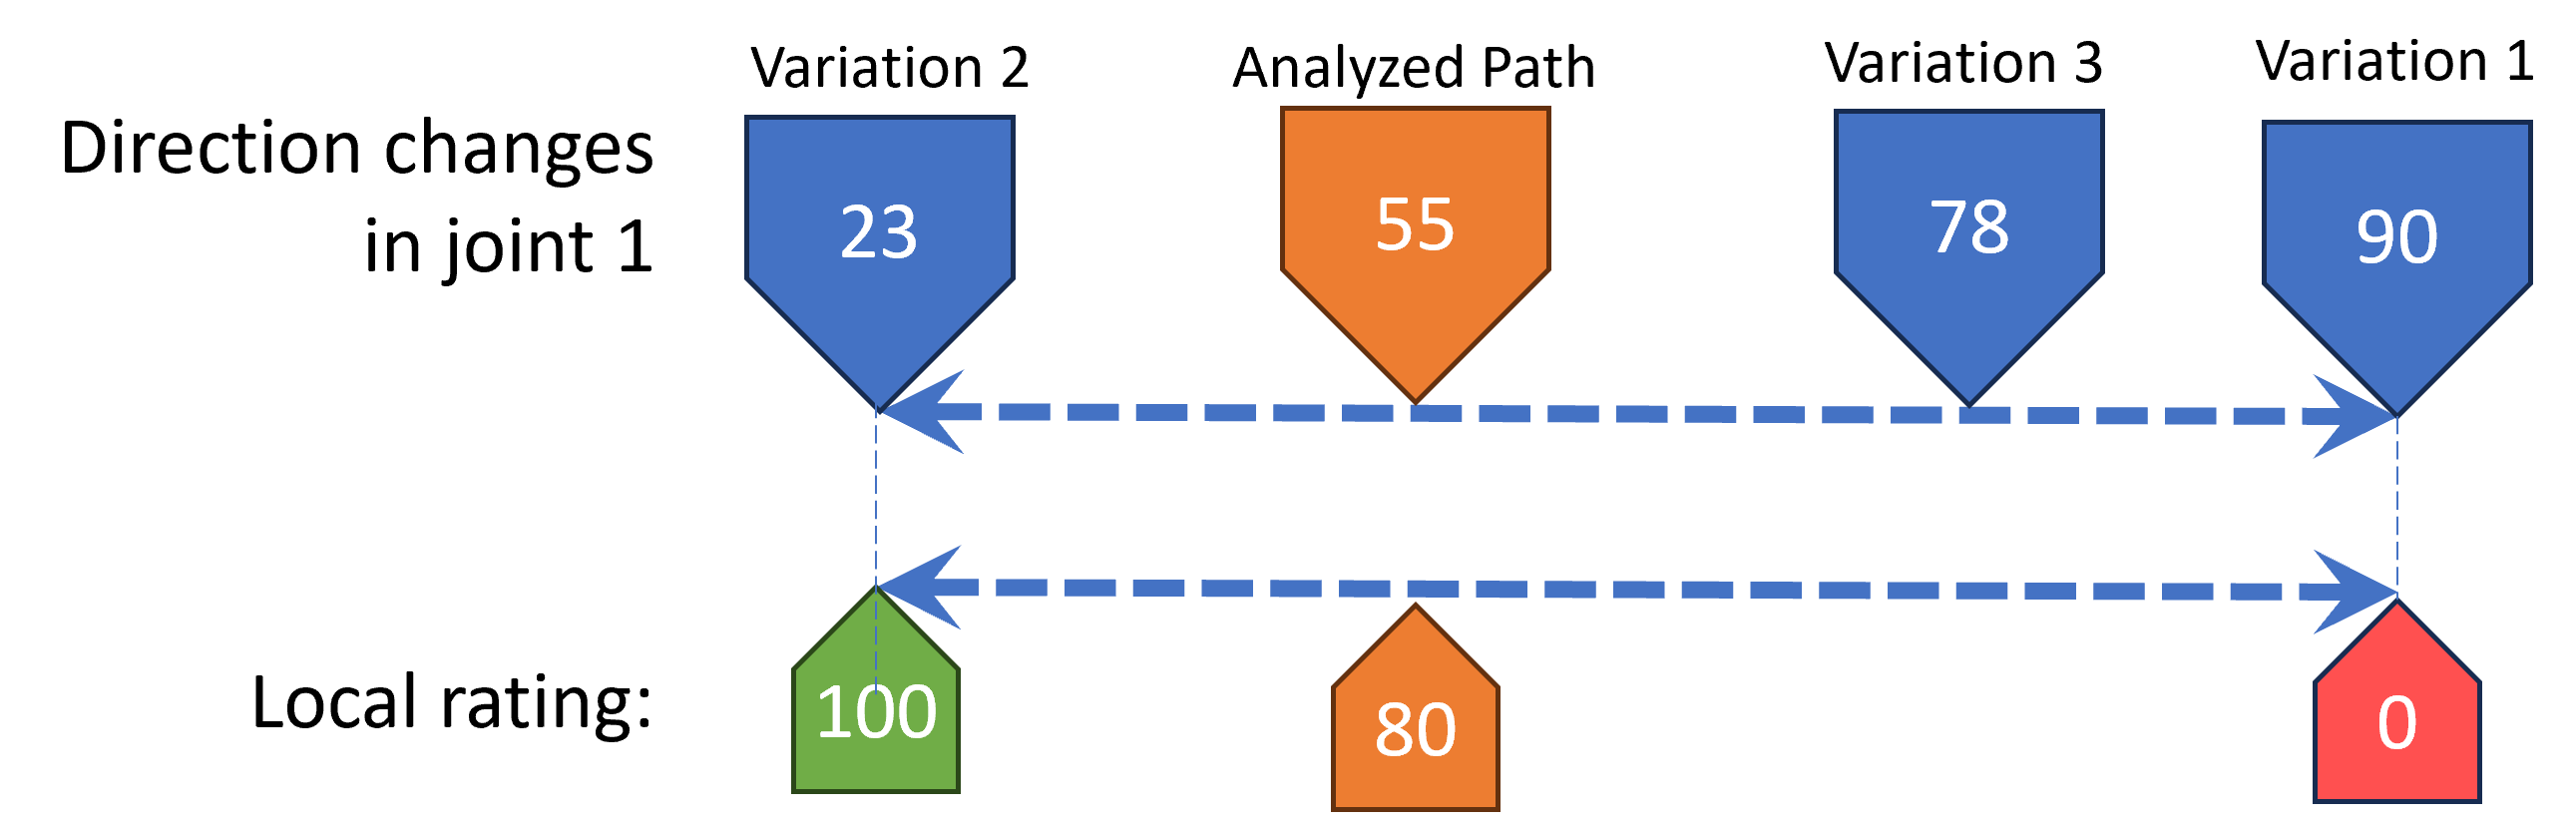
\includegraphics[width=0.85\textwidth]{figures/localscore.png}}
	\caption{Calculation of the local score trough variation}
	\label{Localscore}
\end{figure}
\newpage
It is important to note that increasing the number of variations performed before calculating the local score will enhance the accuracy of this approach. If only a few variations are executed, there is a possibility that only similar outcomes will be found, which significantly affects the result. Furthermore, the user needs to specify whether a high or low scalar value of a process variable is desired. The Min-Max scaler should return the local score accordingly. 

Another factor that needs to be analyzed is whether the variations in the boundary conditions lead to process variable values that exceed a certain standard deviation. Figure~\ref{lowstd} illustrates how a local rating of 66 for the total energy consumption is calculated, despite the presence of very small absolute differences. In this case, the standard deviation is only 0.37.

\begin{figure}[H]
	\centerline{\includegraphics[width=0.85\textwidth]{figures/lowstd.png}}
	\caption{Variation with low standard deviation}
	\label{lowstd}
\end{figure}

 On the other hand, Figure~\ref{highstd} demonstrates how the same local rating of 66 is calculated, even though the absolute differences are significantly higher. Here, the standard deviation is 22.36. The local rating should only be used as input for the local score if the standard deviation exceeds a predetermined threshold. If the standard deviation criteria are not met, the corresponding process variables and its local score should be excluded from the calculation of the global score. In the following chapters, each process variable and its conversion into a single scalar value is discussed in more detail. 

\begin{figure}[H]
	\centerline{
\includegraphics[width=0.85\textwidth]{figures/highstd.png}}
	\caption{Variation with high standard deviation}
	\label{highstd}
\end{figure}

 
\subsection{Information Extraction form Time-Series Data}\label{extraction}
It is important to note that, as discussed in Chapter \ref{LRC}, the computation of a local score requires transforming a time-series into a single scalar value. This transformation can be accomplished by directly manipulating the time-series data, such as summing up all values, or by conducting subsequent analyses. Since each time-series captures distinct physical phenomena, each one necessitates a unique process for converting it into a scalar value.





\section{Information from Angular Position}
In its isolated form, the rotational or angular position of a joint does not provide much information to enable extensive qualitative analysis. However, when supplemented with temporal information, it becomes a valuable source of information. By considering the angular position in conjunction with the temporal dimension, a more comprehensive understanding of joint behavior can be obtained, allowing for more in depth analysis. Figure \ref{agularstuff} visualizes what information needs to be added to enrich the analysis of these process variables that are directly related to the angular position of joints.

\begin{figure}[H]
	\centerline{\includegraphics[width=0.95\textwidth]{figures/angularstuff.png}}
	\caption{Additional information for angular position of each joint}
	\label{agularstuff}
\end{figure}

The first additional required piece of information is the temporal element, which specifies the exact time when a joint should be in a specific rotational position. This information can be recorded in small equidistant time intervals or only record the positional changes. Recording only the change in position is not ideal because it does not accurately represent the physical aspect of the system. In reality, the position cannot change significantly from one time interval to the next. Additionally, this method does not provide information about the rotational velocity at which the joint should change position. On the other hand, continuous recording in small equidistant time intervals can result in a higher number of recorded values and, consequently, a longer time-series.

Figure \ref{equi} illustrates the rotational position of a rotary joint over time in degrees. The left side of the figure illustrates the position recorded with equidistant fine grained time intervals, while the right side displays a time-series where only the destination positions and their corresponding times are recorded. Both series have very similar characteristics but offer a significantly different information content.
\newpage

\begin{figure}[H]
	\centerline{
\includegraphics[width=0.90\textwidth]{figures/equionchange.png}}
	%\caption{Time-series of a rotary joint with equidistant time steps}
	\caption{Two option for recording the joint position in a time-series}
	\label{equi}
\end{figure}

%\begin{figure}[H]
%	\centerline{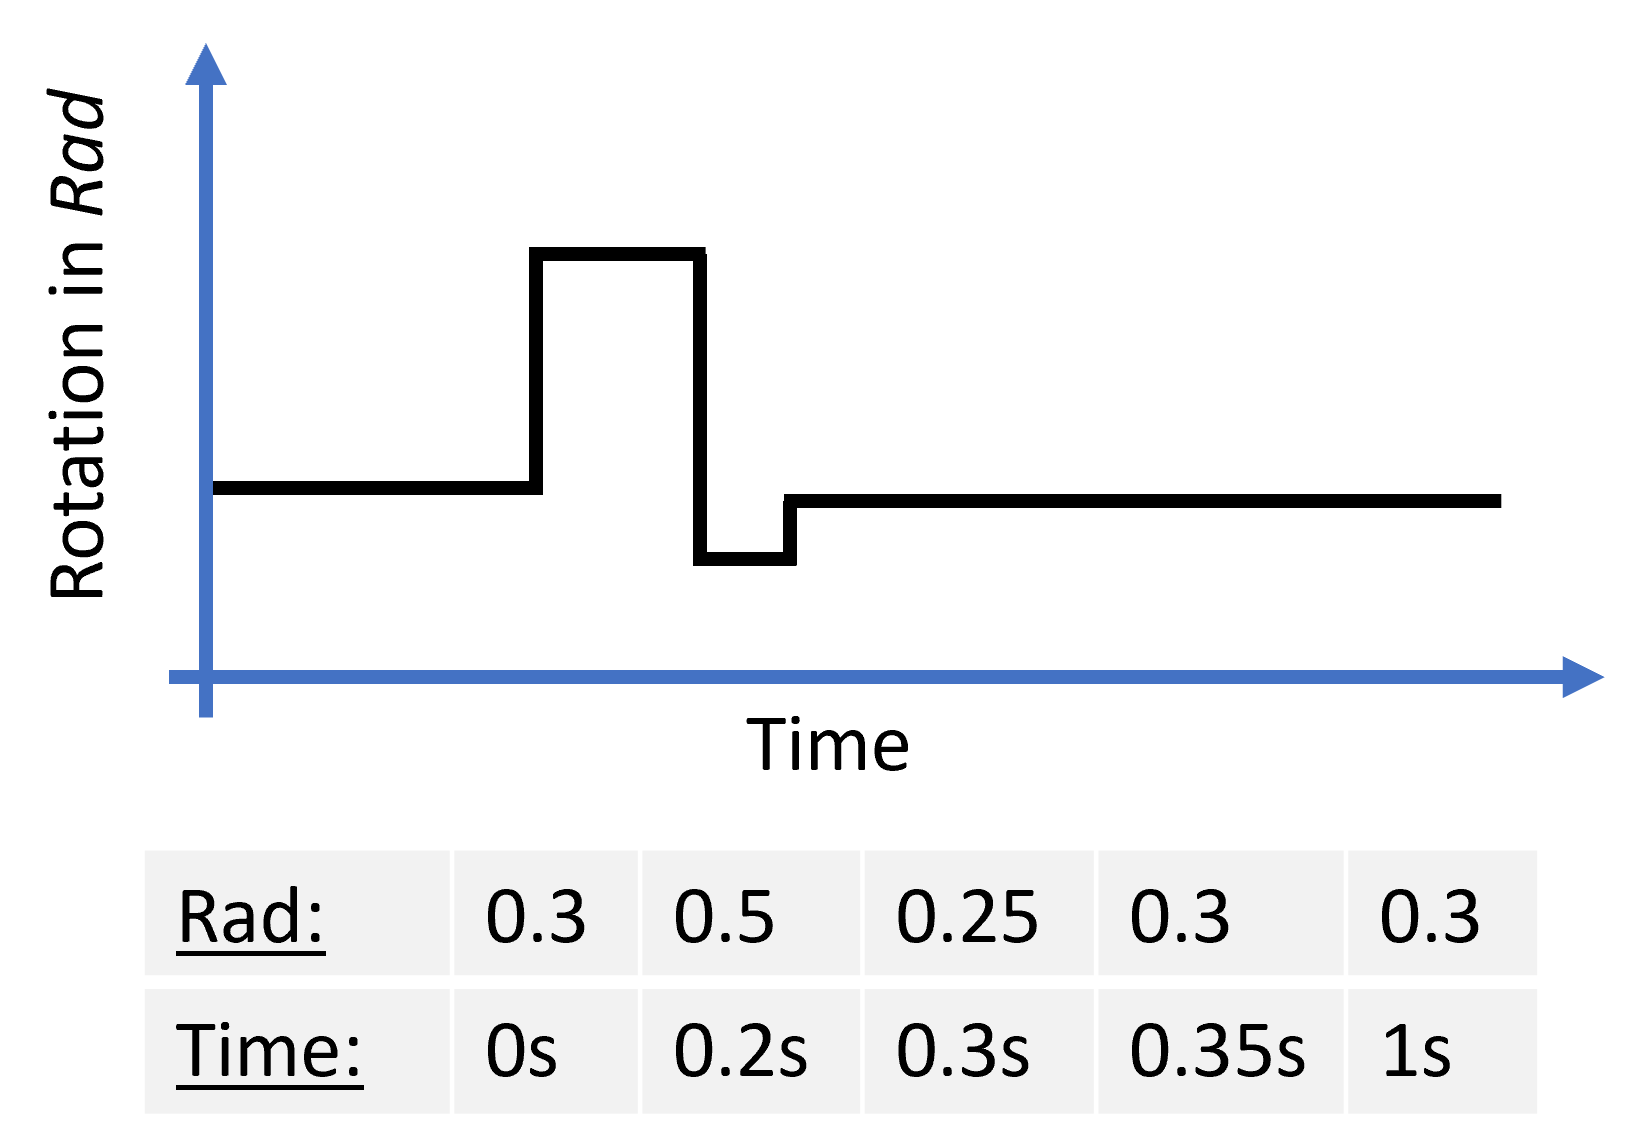
\includegraphics[width=0.5\textwidth]{figures/onchange.png}}
%	\caption{Time-series of a rotary joint with only the recorded end positions}
%	\label{onchange}
%\end{figure}

\subsection{Total Joint Travel and Direction Changes}
Parameters that can be analyzed without the need for any additional information include the number of direction changes and the total travel of a joint. The total travel can be determined by subtracting the position of two consecutive recorded points and summing up the absolute values. Furthermore, additional information can be derived by separately summing up the clockwise and counterclockwise rotations. By combining the absolute values of these rotations, the overall travel of the joint can be obtained.

Figure \ref{travel} provides a visual representation of the calculation of total travel. The total forward rotation (clockwise) can be determined by summing up the lengths of the green arrows, while the total backward rotation (counterclockwise) is obtained by summing up the lengths of the orange arrows.

\begin{figure}[H]
	\centerline{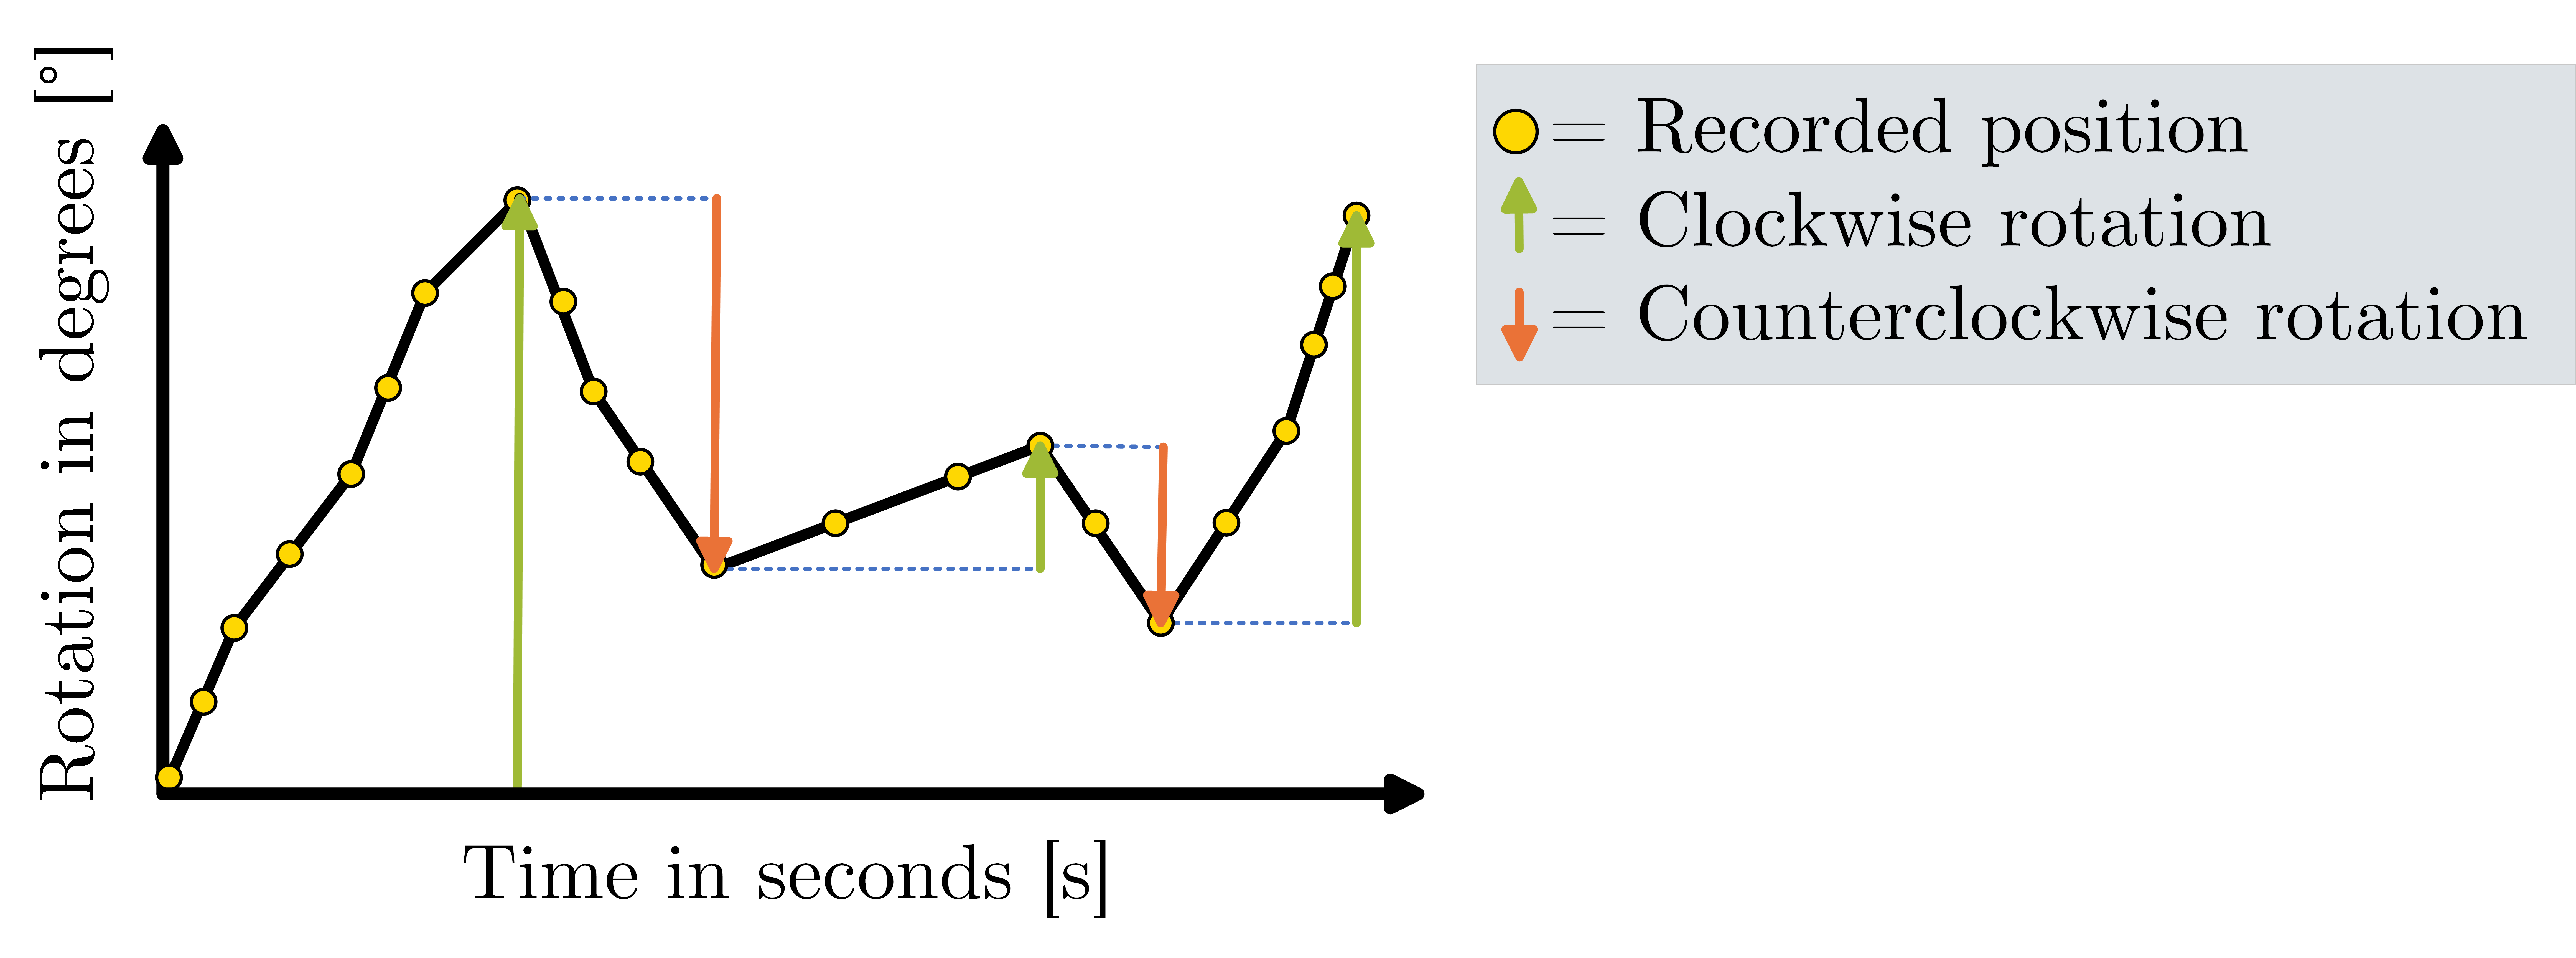
\includegraphics[width=0.8\textwidth]{figures/travel.png}}
	\caption{Summing up the rotation in the clockwise and anti-clockwise direction }
	\label{travel}
\end{figure}

The number of direction changes is a variable that can be determined by analyzing the joint position alone, without the need for temporal information. This can be accomplished by identifying points where the position before and after either decreases or increases. However, it is important to note that this method may not be applicable to points where multiple positions are recorded at the same value consecutively. To address the issue of multiple positions recorded at the same value, a potential solution is to introduce a tracking value that indicates whether the previous change in direction of two consecutive positions was either upward or downward. If the direction of two positions is different from the tracking value, the direction change counter is incremented by 1. However, if the direction is the same as the previous points or if the positions are identical (neutral), the direction change counter and tracking values remain unchanged. Figure \ref{dirchange} provides a visual representation of the points where the direction change counter is incremented.


\begin{figure}[H]
\centerline{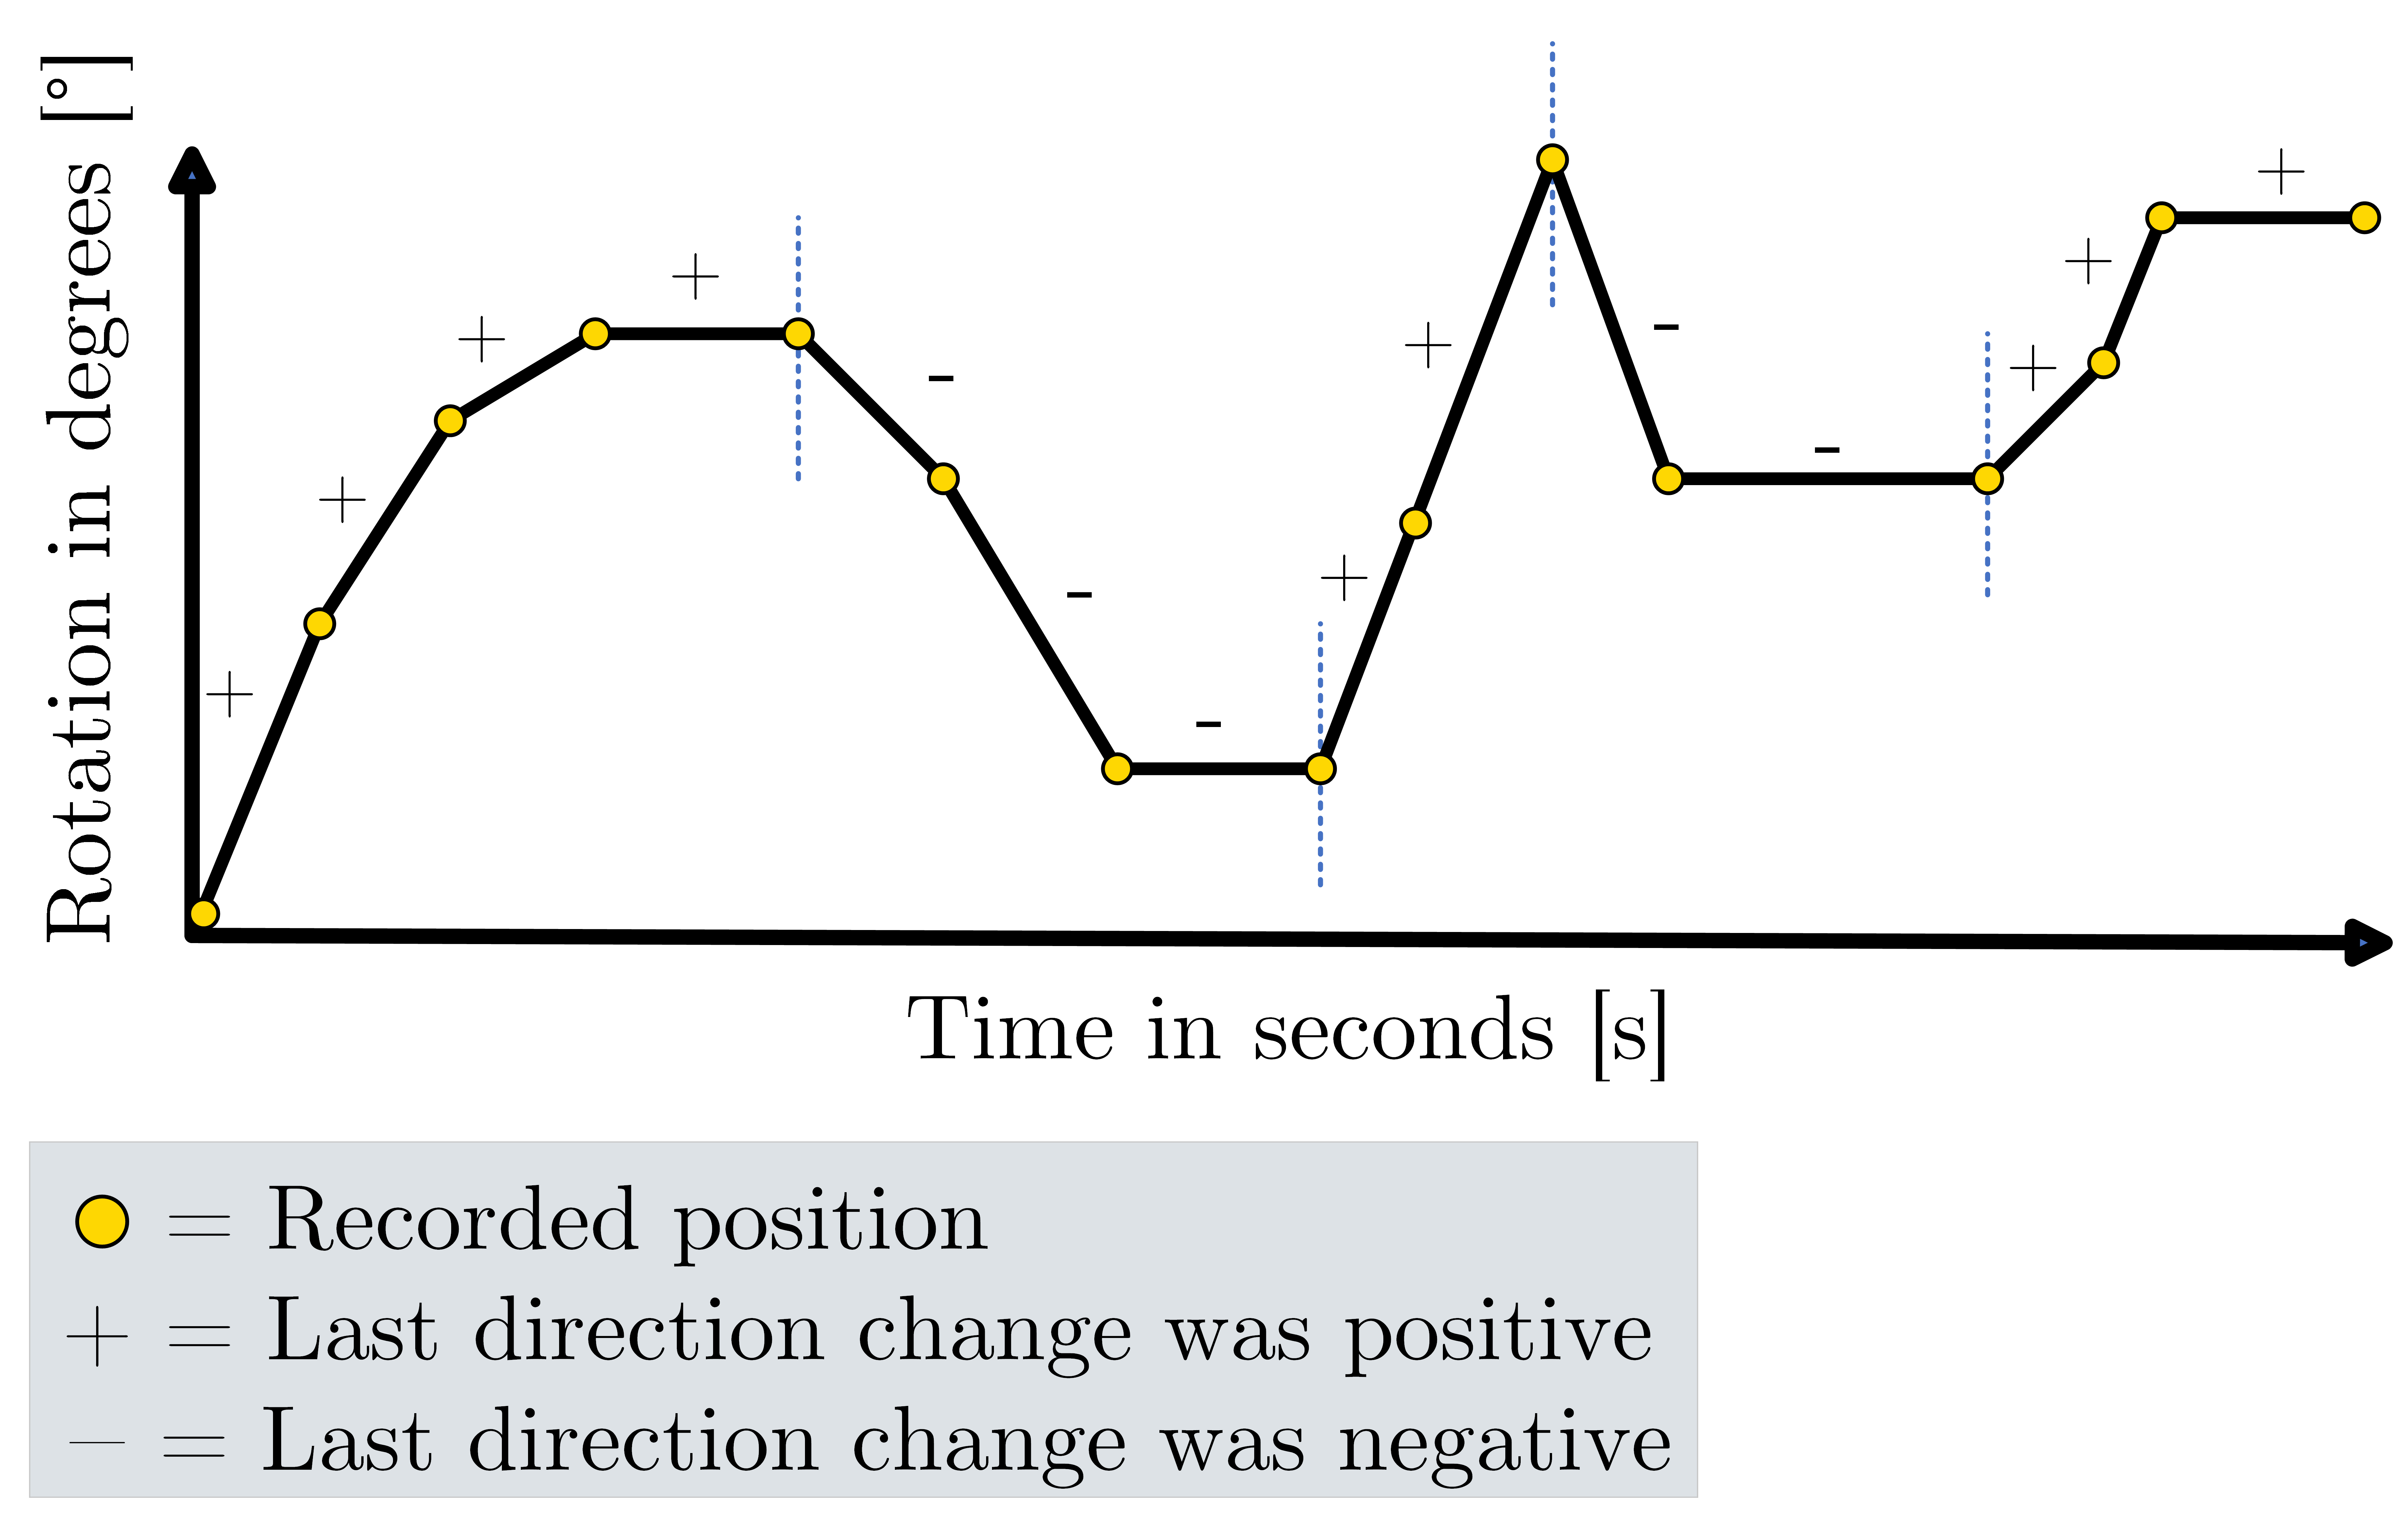
\includegraphics[width=0.7\textwidth]{figures/dirchange.png}}
	\caption{Calculating direction changes from a time-series}
	\label{dirchange}
\end{figure}

The counters for direction changes and total travel of each joint can be easily transformed into a local rating, as explained in Chapter \ref{LRC}. This local rating can then be multiplied by an importance factor to calculate the local score. The direction changes can be summed up over all joints, or they can be specifically grouped based on certain criteria or categories.  

Table \ref{exampleDirTravel} provides an example of how a global score can be calculated based solely on the number of direction changes and total travel. The table illustrates how different joints and variables can be weighted and grouped together to calculate the global score. By assigning different importance factors to each variable, the overall global score can reflect the desired optimum. It is important to note that only the local ratings are multiplied by the importance factor, not the actual counted direction changes or total travel values, to form the local scores. This allows the local score to range from 0 to 100. In this example, due to the high local rating and importance factor for the direction changes in joint 1, the overall global score is also very high. This clearly shows the significance of the importance factors in the calculation of the scores.
\newpage

\begin{table}[H]
	\centering
	\begin{tabular}{||l|r|r|r||}
		Process variables & Local rating & Importance & Local score\\
		\hline
		\hline
		\hline
		
		Direction changes in joint 1 & 95 & 0.7 & 66.5\\
		Direction changes in joint 2-6 & 45& 0.1&4.5\\
		Total travel in joint 4& 34& 0.1&3.4\\
		Total travel in joint 1-3 and 5-6& 46&0.1&4.6\\
		\hline
		\hline
		\hline
		Global Score& & &79\\
		\hline
		\hline
	\end{tabular}
	
	\caption{Calculation of a score regarding only direction changes and total travel}
	\label{exampleDirTravel}
\end{table}


In certain cases, adjusting the boundary conditions may not be sufficient to reduce the number of direction changes, but can offer an improvement in a different area. It is important to note that having the same number of direction changes does not necessarily mean that two time-series are identical. Figure \ref{dirchangeSTD} visually demonstrates two time-series with the same number of direction changes but distinct characteristics.

\begin{figure}[H]
	\centerline{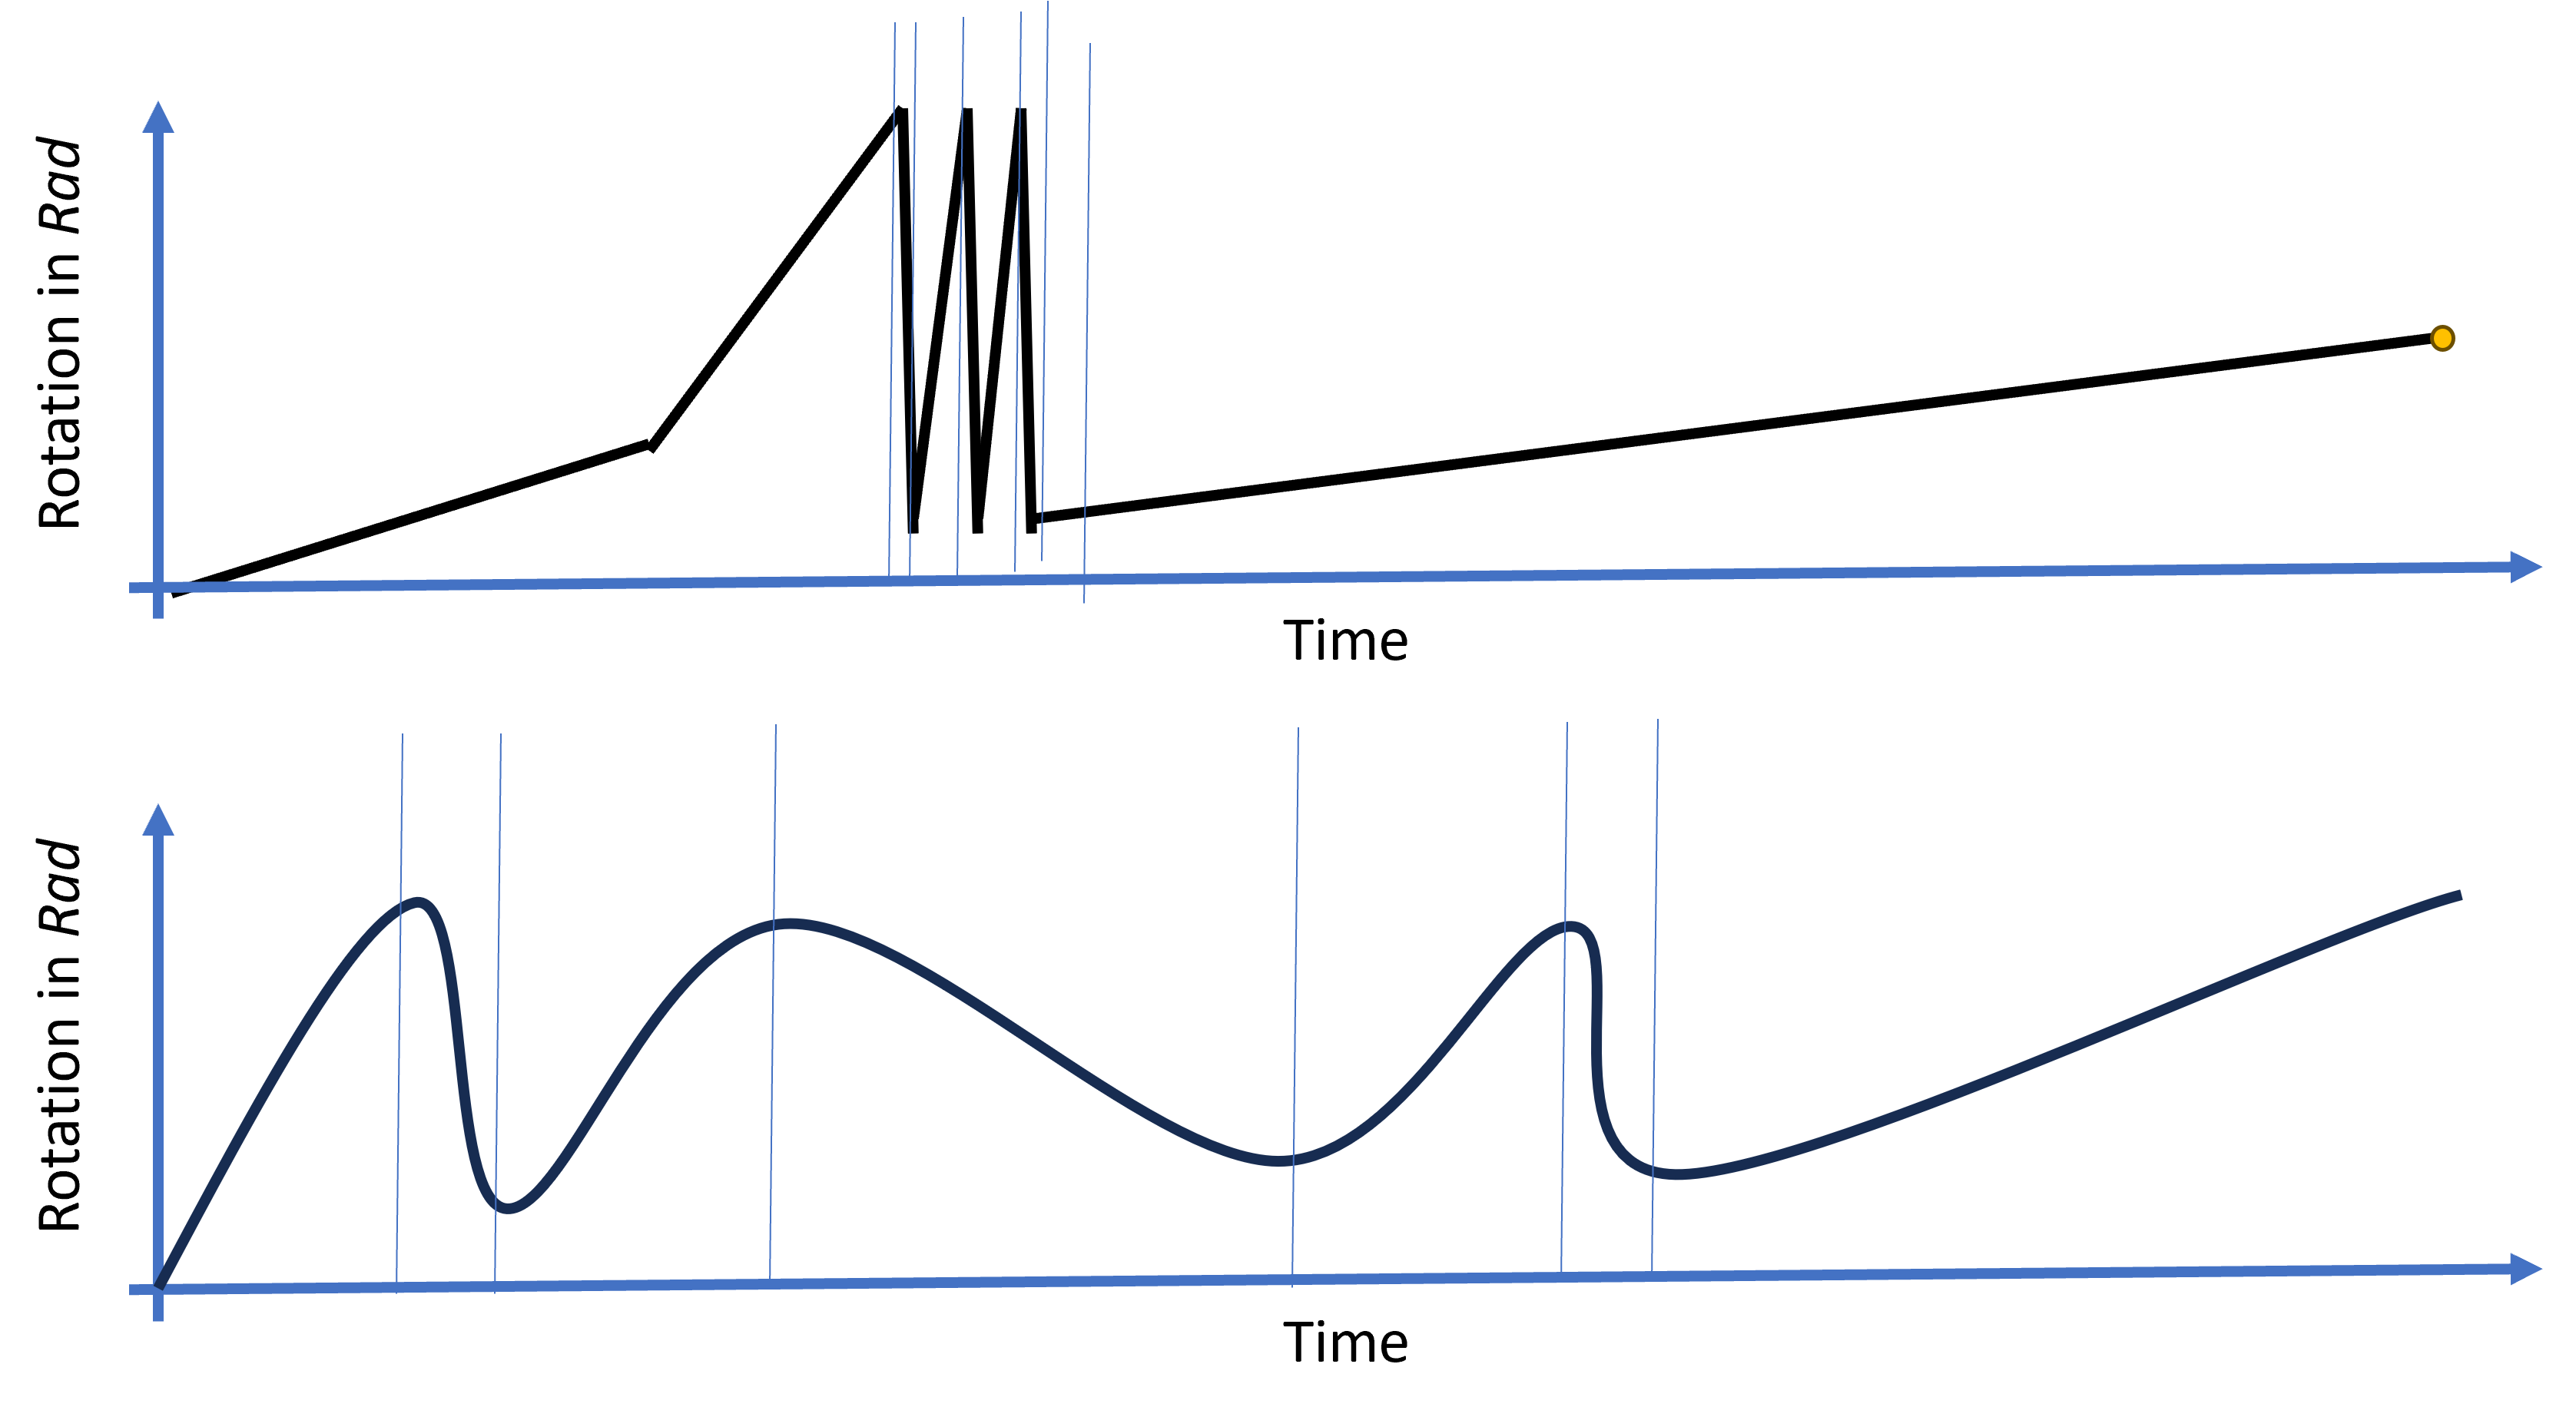
\includegraphics[width=0.75\textwidth]{figures/DirSTD.png}}
	\caption{Two time-series with equal number of direction changes but different characteristics}
	\label{dirchangeSTD}
\end{figure}

To distinguish between these cases, the standard deviation can be utilized. By incorporating the standard deviation, toolpaths that result in frequent and closely spaced direction changes can be identified and are generally considered less desirable. By combining the factor of standard deviation with the number of direction changes, they can be integrated into a single variable. This can be achieved by dividing the number of direction changes by the standard deviation. %By incorporating this calculation and the variation-approach, a local score can be determined.
This approach provides an evaluation method that takes into account both the quantity of direction changes and the variability within the time-series data. When there are only a few direction changes but with a high variance, the resulting variable value will be very low. Conversely, when there are numerous direction changes but with a low variance, the variable value will be high.




\subsection{Rotation Limits}\label{RotLim}
Additionally, a straightforward analysis of rotational limits can be conducted, requiring knowledge of four distinct values. The first two values are the upper and lower physical limit that a joint cannot exceed, as surpassing those limit can cause significant damage to the robot. The other two values are potential soft limits put in place to prevent over-rotation of the joint beyond its physical limits. To validate whether any joint positions approach or exceed these limits, a simple comparison of all values can be performed. In cases where it is known that a joint is most stable within a specific range, additional limits can be defined accordingly.

Once a toolpath with defined boundary conditions is established, the joint angles can be analyzed through a simple comparison process. If the joint positions exceed the soft limits or deviate excessively from the desired orientation, a "No-Go" exception is triggered. It is important to note that the analysis of rotation limits does not contribute to the calculation of the global score but serves as a validity assessment to determine if the required movement for the toolpath is physically feasible.

Figure \ref{limits} visually illustrates an example of how the analysis includes the hard and soft limits, as well as the desired position range, of a specific joint. If the limits are not exceeded, the toolpath with the set boundary conditions is deemed safe to be executed. At each time step, the amount by which the joint exceeds the desired area can be summed up to form a scalar value, which can then be used to calculate the local score. By doing so, the toolpath with the most optimal boundary conditions will ensure that the joint positions remain within the desired area.

\begin{figure}[H]
	\centerline{\includegraphics[width=0.9\textwidth]{figures/limits.png}}
	\caption{Hard and soft limits with desired range}
	\label{limits}
\end{figure}

\subsection{Velocity, Acceleration and Jerk of the Joints}\label{VAJJ}
To conduct a specific analysis of the rotational velocity, acceleration, and jerk of the joints, a time derivative needs to be applied. By performing simple comparisons of the time-series values, it becomes possible to determine whether the maximum capabilities of the motor driving the joint are being exceeded.

Figure \ref{velo} demonstrates how the velocity aspect can be transformed into a scalar value, which can then be utilized in the calculation of a local rating. Firstly, the joint velocity is obtained by taking the absolute time derivative of the joint position. Subsequently, an analysis is conducted to determine the duration for which the absolute velocity exceeds a certain threshold value. In the given example, the threshold is set at 80\%. 

\begin{figure}[H]
	\centerline{\includegraphics[width=1\textwidth]{figures/veloy.png}}
	\caption{Calculating velocity from the joint position over time}
	\label{velo}
\end{figure}

Additionally, it is feasible to incorporate multiple thresholds and assign linear or exponential weights to them relative to each other. The combined outcome is then utilized to calculate the local score. For example, if the 80\%-threshold is exceeded for 15 seconds and the 90\% threshold is exceeded for 5 seconds, the a scalar value is calculated by multiplying the corresponding time and threshold and summing them up. In this case the result is 80~*~15~+~90~*~5~=~1650.

It is also possible to determine whether a short but significant peak over the threshold values is more desirable than a constant but small overstep. Figure \ref{peaklong} provides a visualization of these two cases.

\begin{figure}[H]
	\centerline{
\includegraphics[width=1\textwidth]{figures/peaklong.png}}
	\caption{Overstepping the threshold value}
	\label{peaklong}
\end{figure}
\newpage
In the former case, where peaks are more desirable, it is sufficient to sum up the area between the velocity and the set threshold. If avoiding peaks is the top priority, all elements in the velocity time series can be cubed and summed up. By cubing the values, peaks will be exponentially weighted, making them easier to optimize for.


The simplest approach, however, is to square all values and take the sum. This method eliminates the need to define multiple threshold boundaries. Additionally, high peaks will have a greater impact on the resulting value compared to small, constant values, without overshadowing the final result. If the velocity exceeds the maximum velocity, a "No-Go" exception must be triggered, indicating that the movement is not possible. The same rating principle can be applied to acceleration and jerk. Acceleration is obtained by taking the derivative of velocity, while jerk is obtained by taking the second derivative. Individual limits and thresholds can be set to determine the optimality of the robot's movement. If the maximum acceleration or jerk is exceeded, a "No-Go" error is also triggered.

Table \ref{VAJ} presents the calculation of a global score, which incorporates a weighting that prioritizes low acceleration in joint 2 and allows for high velocity in all joints. The acceleration in joint 1 and joints 3 to 6 are considered to be of lesser significance. The jerk is completely omitted from the rating in this example. Due to the close-to-optimal acceleration in joint 2 and its high importance value, the overall score of the toolpath with the defined boundary condition is also very good.

\begin{table}[H]
	\centering
	\begin{tabular}{||l|r|r|r||}
		Process Parameters & Local rating & Importance & Local score\\
		\hline
		\hline
		\hline
		Velocity in Joints 1-6& 45& 0.1&4.5\\
		Accelerations in Joint 2& 90 & 0.8 & 72\\
		Accelerations in Joint 1 and 3-6 & 15& 0.1&1.5\\
		Jerk in joints 1-6& 4& 0&0\\
		
		\hline
		\hline
		\hline
		Global Score& & &78\\
		\hline
		\hline
	\end{tabular}
	
	\caption{Calculation of a score regarding only velocity, acceleration and jerk}
	\label{VAJ}
\end{table}

\begin{comment}
\section{TCP Coordinates, Velocity and Acceleration}\label{CVA}
As discussed in Chapter \ref{pp}, the forward kinematics approach allows for the calculation of the \acrshort{TCP}'s X,Y and Z coordinates as well as orientation. Alternatively, this information can be directly extracted from the G-code.

By calculating the time derivative of the positions, it is possible to determine both the velocity and acceleration of the \acrshort{TCP}. These variables play a significant role in milling applications, particularly when precise corners need to be fabricated. It is important to note that both robotic systems and \acrshort{CNC} machines have limitations on their acceleration capabilities. As highlighted in Chapter \ref{CPM}, these limitations result in slight deviations occurring in the path, especially at corners. These deviations arise from the systems' inability to instantaneously change velocity or direction. Consequently, the \acrshort{TCP}'s path will not be perfectly followed as demanded by the G-Code and will exhibit minor variations in the corners.

To quantitatively analyze the magnitude and frequency of these deviations, it is crucial to examine the start and endpoints of the linear toolpath as defined in the G-code. When the endpoints are aligned along a vector in space, it indicates that no deviation from the desired toolpath is expected. However, a misalignment between the endpoints suggests an anticipated deviation.

Figure \ref{devi} gives a visual example of the position in th X-Y plane that the robot needs to traverse. The expected deviation is shown in red.

\begin{figure}[H]
	\centerline{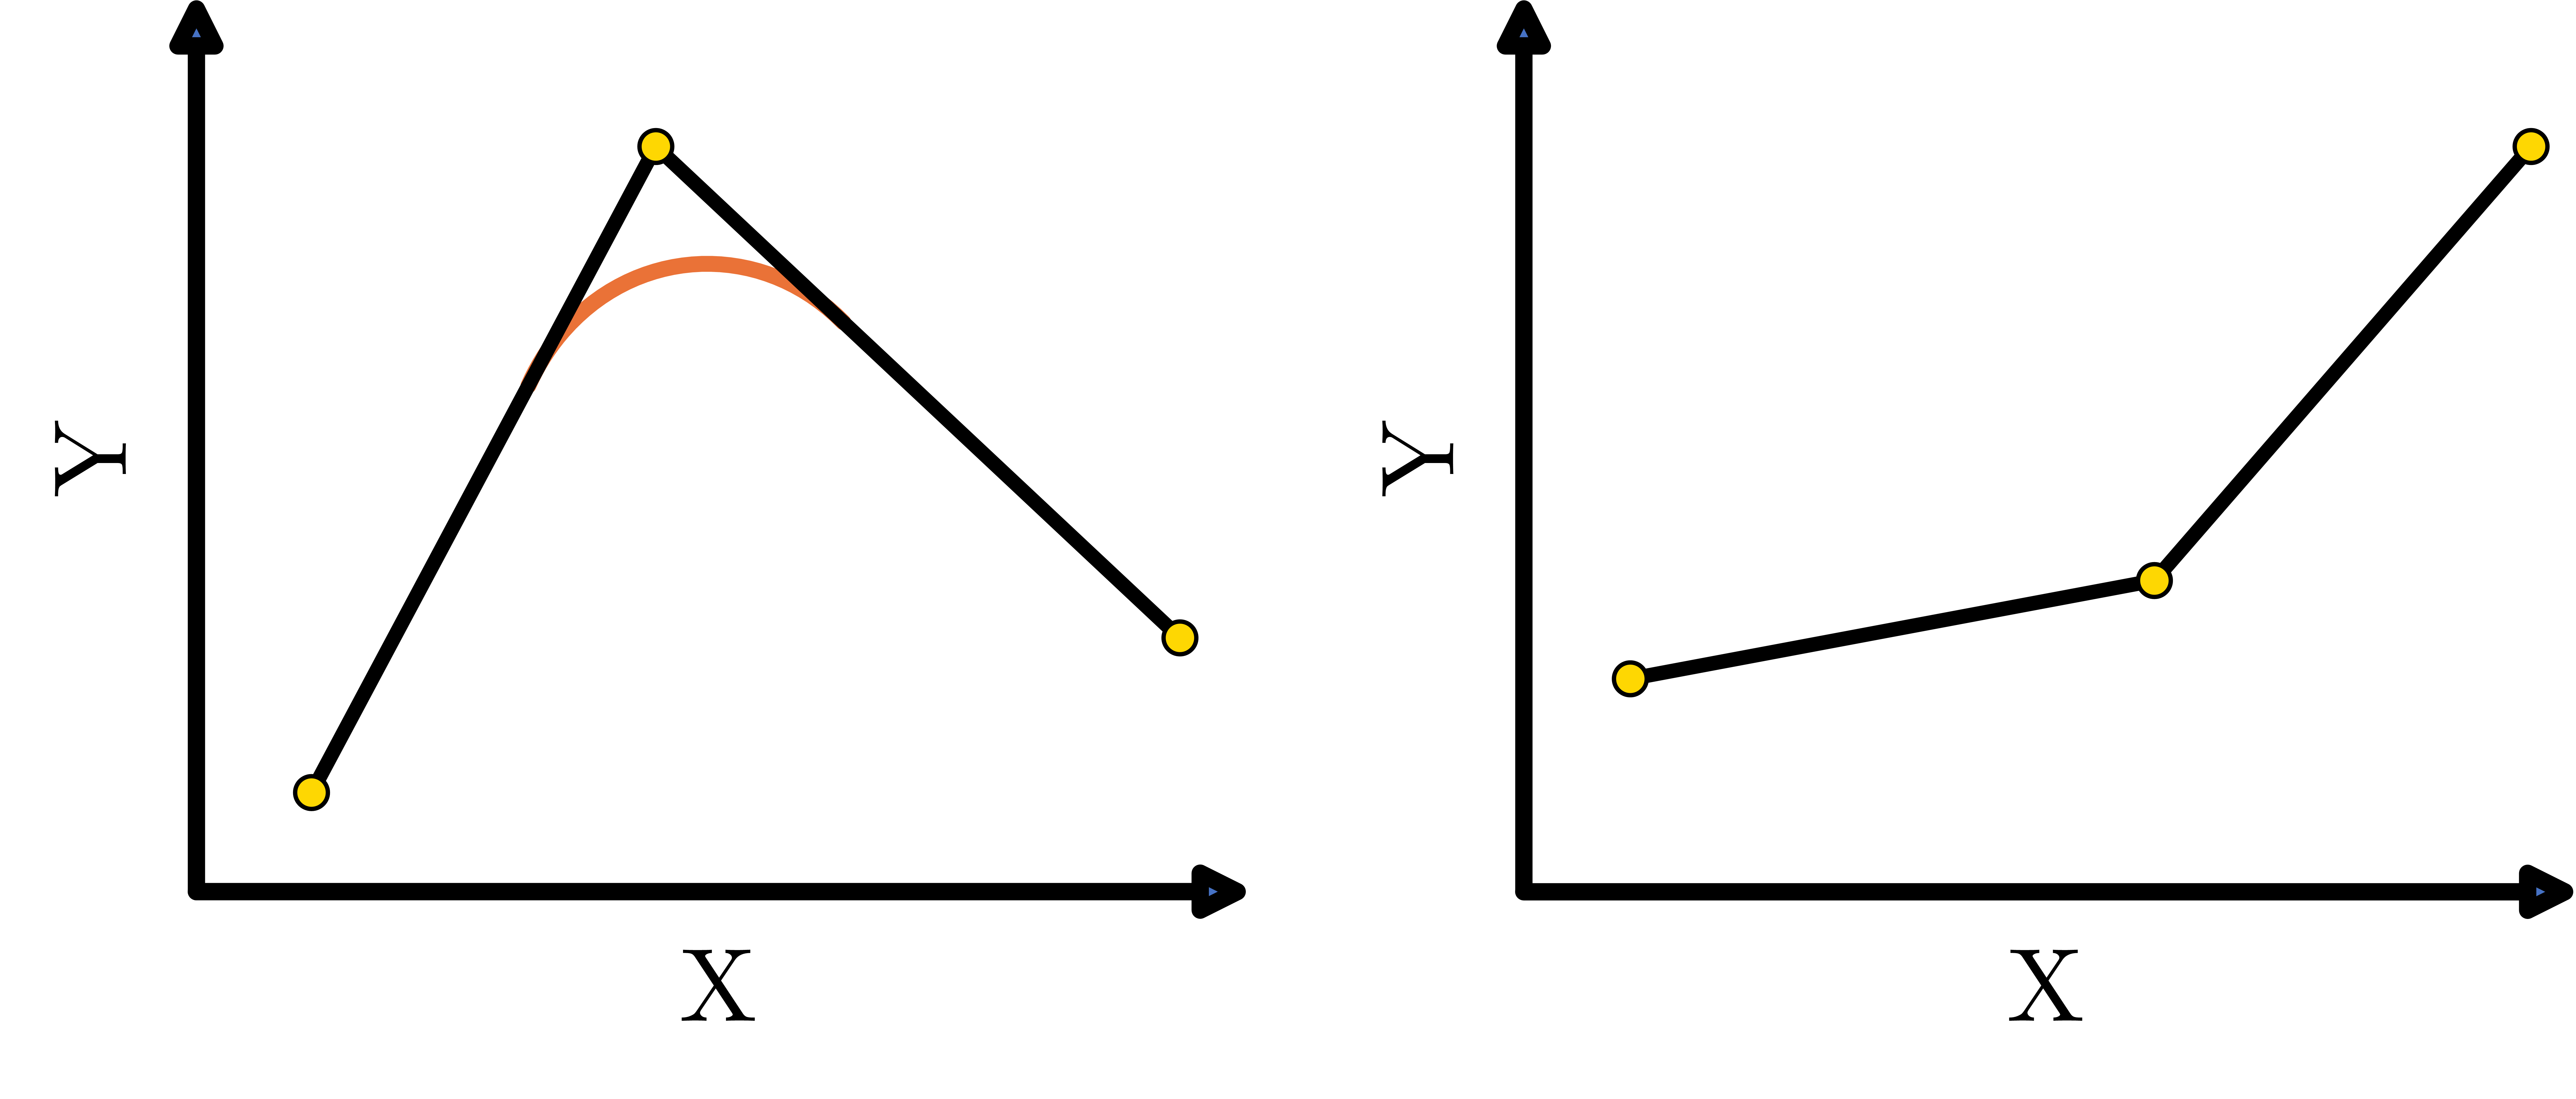
\includegraphics[width=.5\textwidth]{figures/uber.png}}
	\caption{Deviation of of the TCP from the actual toolpath}
	\label{devi}
\end{figure}

In order to obtain a qualitative estimate of the total deviation, it is necessary to additionally analyze the individual velocity vectors that characterize the toolpath. Perfect alignment of the velocity vectors indicates no expected deviation. However, as the angle between consecutive velocity vectors increases, the deviation also increases. To quantitatively represent this information, the sine of each angle can be calculated and summed. An angle of 0 or 180 degrees will result in a value of 0, while an angle of 90 degrees will yield a value of 1. This scalar value provides an indication of the overall magnitude of the expected deviation.

%Additionally, it is crucial to consider the magnitude or speed of the velocity vectors. In cases involving sharp corners with high velocities, the deviation is anticipated to be more significant compared to corners with lower velocities. To account for this, the result obtained from the sine calculation can be multiplied by the smaller of the two velocities. 

%This analysis is useful for operators in defining more optimal machining strategies~(see~Chapter~\ref{papla}). 

In the context of \acrshort{WAAM}, the acceleration of the welding torch plays a crucial role in the process. This is particularly evident when utilizing \acrshort{CMT} technology, which involves wire retraction, as discussed in Chapter \ref{CMTc}. A rapid acceleration of the welding torch can lead to unintended drop detachment and imprecise drop placement. Consequently, the quality and accuracy of the additive manufacturing process may be compromised, resulting in defects and deviations from the desired geometry.

However, it is worth noting that, similar to the deviation in the toolpath discussed earlier, this issue cannot be directly optimized by simply defining specific boundary conditions in the form of redundant \acrshort{DoF}.

\section{Energy Usage}
Energy usage is a critical factor in modern manufacturing. To minimize unnecessary and energy-intensive movements, it is crucial to select appropriate boundary conditions for the additional constraint . The analysis of energy usage can be approached in two distinct ways.

Firstly, a continuous energy analysis allows for the attribution of specific energy consumption to each movement. This approach provides detailed insights into the energy usage of individual actions or operations. Secondly, considering the overall energy requirement throughout the entire manufacturing process provides a holistic perspective on energy utilization. This approach allows for optimizing energy usage and making informed decisions regarding energy efficiency in manufacturing.
\end{comment}
\subsection{Continuous Energy Usage}
Tracking energy consumption can be achieved through a straightforward method of monitoring the velocity and acceleration of individual joints. The energy demand is composed of two components: the rotational movement of a joint at a predetermined speed and the joint's acceleration.

To determine the energy consumed by each joint, the time-series data of joint velocity and acceleration can be multiplied by the average energy consumption value, either in \(\frac{\si[per-mode=symbol]{\kWh}}{\si[per-mode=symbol]{\m\per\sec }}\) or \(\frac{\si[per-mode=symbol]{\kWh}}{\si[per-mode=symbol]{\m\per\sec\squared }}\), associated with that particular joint. By summing up these resultant time-series, an energy consumption profile for each joint can be obtained. The newly obtained time-series represent the energy consumption to move from one pose to another. Aggregating the time-series data from all joints into one time-series provides an overall estimation of the robot's energy consumption. %Table \ref{scalers} gives exemplary values for the scaling factors.
\begin{comment}
\begin{table}[H]
	\centering
	\begin{tabular}{||l|r|r||}
		Joint Nr.  & Velocity Scaling Factor in \(\frac{\si[per-mode=symbol]{\kWh}}{\si[per-mode=symbol]{\m\per\sec }}\)& Acceleration Scaling Factor in \(\frac{\si[per-mode=symbol]{\kWh}}{\si[per-mode=symbol]{\m\per\sec\squared }}\) \\
		\hline
		\hline
		\hline
		Joint 1	& 0.1 & 0.5\\
		Joint 2	&  0.4& 0.3 \\
		Joint 3	& 0.3& 0.2\\
		...& ...& ...\\
		
		\hline
		\hline
	\end{tabular}
	
	\caption{Average scaling factors for energy calculations}
	\label{scalers}
\end{table}
\end{comment}
This approach offers a notable advantage in its simplicity. Nevertheless, its primary limitation stems from the potential inaccuracies that may arise when working with an average scaling value. If this value is derived by averaging all possible positions, but only a limited number of positions are actually traversed by the robot, significant discrepancies can occur.


To address these limitations, more advanced approaches are necessary. For instance, the utilization of multi-body simulations (\acrshort{MBS}) in \acrshort{CAM} software enables a direct analysis of the exact energy requirements for a robot to move between different poses. This method requires precise modeling of weight distribution to achieve accurate outcomes. However, it is important to consider that implementing this approach may require substantial computation and development time.


Another viable option to consider, is the utilization of a \acrshort{ML} approach for estimating energy consumption during transitions between discrete poses. By employing a supervised learning technique, where the input data includes the current joint positions and velocities as well as the target pose, an \acrshort{ML} model can be trained to predict the energy required for each transition. This approach offers the advantage of leveraging \acrshort{ML} algorithms to provide accurate energy consumption estimates in a more efficient manner. However, it is important to note that generating high-quality training data and training the \acrshort{ML} model can be a time-intensive processes.

Figure \ref{ENERGYOPTIONS} illustrates the three aforementioned options along with their key requirements. It is important to note that these examples only give an excerpt on how to get an energy estimation and do not cover all possible solutions to address this problem. 

\begin{figure}[H]
	\centerline{\includegraphics[width=1\textwidth]{figures/ENERGYOPTIONS.png}}
	\caption{Exemplary methods for energy usage calculations}
	\label{ENERGYOPTIONS}
\end{figure}
\newpage
Once the time-series data for energy consumption is obtained, it becomes possible to identify peaks and associate them with specific movements. In line with the optimization objective, it is also feasible to establish threshold values, as discussed in Chapter \ref{CVA}, to optimize for a constant energy consumption.


\subsection{Total Energy Usage}
When the aim is to obtain a single scalar value for the total energy consumption, the same procedures outlined in the preceding chapter can be applied, and the values from the time-series can be aggregated through summation.

In situations where the temporal information in energy consumption is considered irrelevant, alternative \acrshort{ML} approaches can be employed. For example, Recurrent neural-networks (\acrshort{RNN}s) can be utilized, as they have the ability to take an entire time-series as input and generate a scalar value representing the total energy consumption. \acrshort{RNN}s excel at capturing dependencies and patterns in sequential data. By training an \acrshort{RNN} model using a time-series dataset, it can learn to predict the total energy consumption based on the provided input. However, it is important to note that, like most \acrshort{ML} approaches, this method requires substantial effort and time for generating training data and conducting the training process.

In \acrshort{WAAM}, it is important to consider the energy consumption associated with the welding process itself. The determination of energy use in welding involves various factors. The G-code, which comprises instructions for the welding process, can provide information on the wire-feed, voltage and the desired power input. By analyzing this code, it becomes possible to estimate the energy consumption during each welding operation. Alternatively, these parameters are often pre-defined as constants on the welding appliance, with the G-code solely specifying the turn-on and turn-off points. Figure \ref{waamgcode} gives an example on how the turn-on (N10) and turn-off points (N70) can be defined in the G-code.
 
\begin{figure}[H]
	\centerline{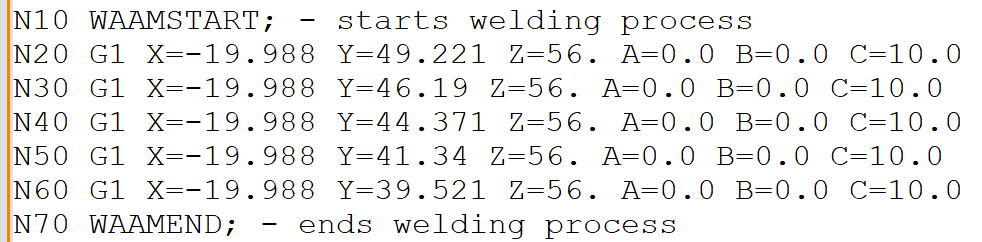
\includegraphics[width=.75\textwidth]{figures/waamgcode.png}}
	\caption{Turn-on and turn-off points in the G-code used in WAAM}
	\label{waamgcode}
\end{figure}

By considering these factors, it is possible to accurately assess the energy usage during welding operations. However, this specific part of the total energy consumption cannot be optimized by defining the boundary conditions of redundant \acrshort{DoF}s. The energy required for the welding process is solely defined by the welding parameters and the final part geometry.

\newpage
\section{Reach, Singularities and Torch Orientation}
The following discusses the robot poses with respect to reach and alignment, singularity avoidance, and torch orientation. These factors are essential in ensuring successful and efficient robotic operations.

\subsection{Reach and Alignment}\label{RO}

As mentioned in Chapter \ref{pp}, the analysis of the reachability index can be conducted in various formats. The first format involves a simple analysis to determine if all the points that the robot needs to traverse, lie within its work volume without any self-collisions or exceeding the soft and hard joint limits. This aspect is closely related to the joint limits, as discussed in Chapter \ref{RotLim}. Additionally, it is necessary to analyze that there are no collisions between the robot and the workpiece. If all these conditions are met, a binary index can be used to indicate the feasibility and safety of executing the program. However, this index cannot be used for optimizing the robot's movement, as the parameters influencing this index are mostly defined by the G-Code.

When utilizing a robotic system with a specific tool, such as a milling spindle or a welding torch for \acrshort{WAAM}, it is crucial to consider the boundary conditions and limits associated with that tool. Figure \ref{rot} illustrates a case where the rotation around the Z-axis of the welding torch can be manually defined. Each positions leads to different strains on the wire-feed system and power-cables.

\begin{figure}[H]%
	\centering
	\subfloat[\centering No rotation]{{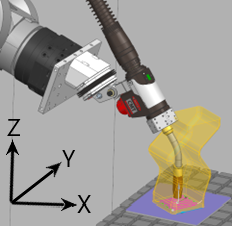
\includegraphics[width=.35\textwidth]{figures/rot0.png} }}%
	\qquad
	\subfloat[\centering 30 degree rotation]{{ 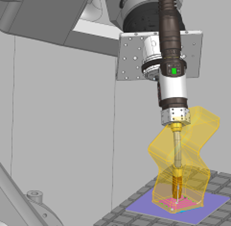
\includegraphics[width=.35\textwidth]{figures/rot1.png}}}%
	\caption{Rotation around the C-axis of a welding torch }%
	\label{rot}%
\end{figure}

In most cases, the spindle and welding torch come with cables that provide power from an external power supply. These cables have an optimal orientation where bending and wear are minimized. By positioning the cables in an optimal orientation, the robotic system can operate efficiently and effectively without any interference or limitations due to cable movement, potential damage, or excessive bending or twisting. To assess the optimality of the robot's cable pose, it is important to consider additional information. In certain cases, it is preferable to route the cables in a specific alignment along a spatial vector, allowing for parallel translation or movement in the direction of that vector. In this case, the angle between the planes of the robot's base coordinate system and the optimal translation vector remains constant. Figure \ref{OOPti}a provides a visual representation of this example. The wire, shown in red, has an optimal alignment along a vector where the least amount of strain is present. Any position along that vector where the cable transitions to the welding torch tangentially is considered optimal. It is worth noting that this vector can be translated parallel in space while still maintaining its optimal status.

In other scenarios, it is more optimal to route the cables towards a specific point in space, such as a mounting point on a wall or ceiling. Figure \ref{OOPti}b illustrates an example where the optimal alignment of a milling spindle is directed towards a designated point where the cables originate. In this case, any position is considered optimal as long as the extended spindle vector aligns with the vanishing point.
\newpage

\begin{figure}[H]%
	\centering
	\subfloat[\centering Optimal alignment along a vector ]{{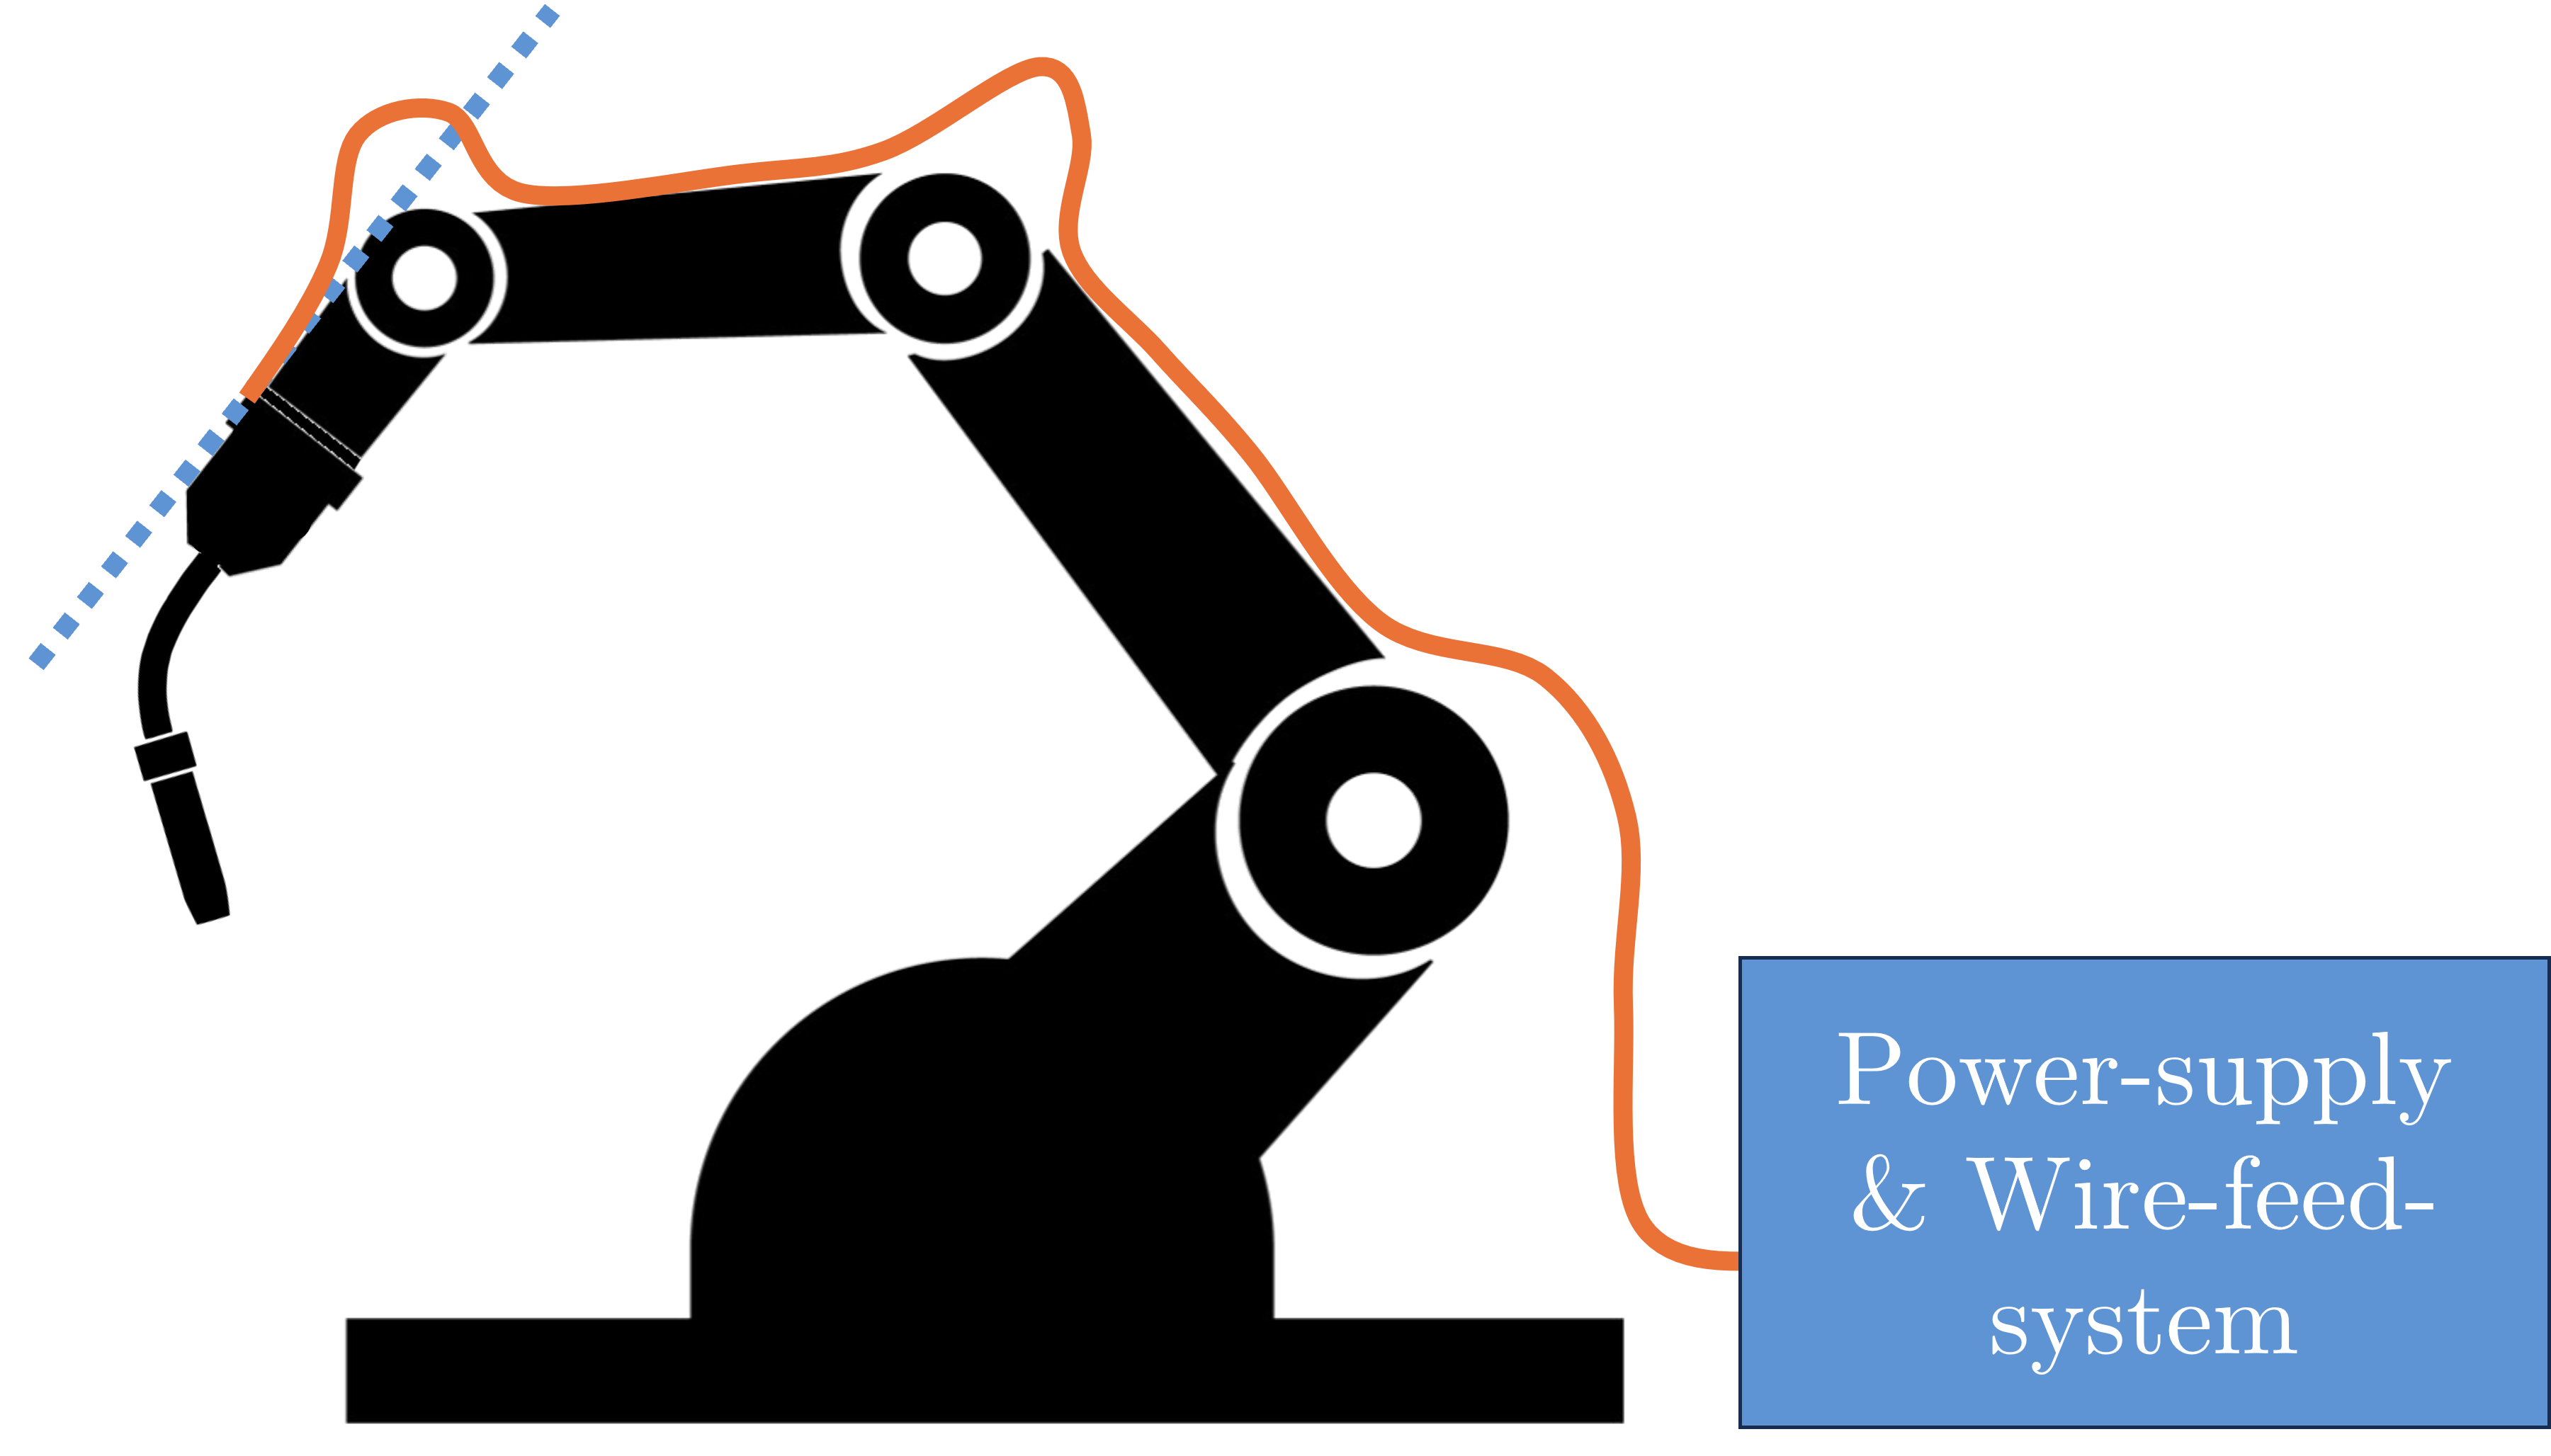
\includegraphics[width=.5\textwidth]{figures/paralell.png} }}%
	\qquad
	\subfloat[\centering Optimal alignment towards a vanishing point ]{{ 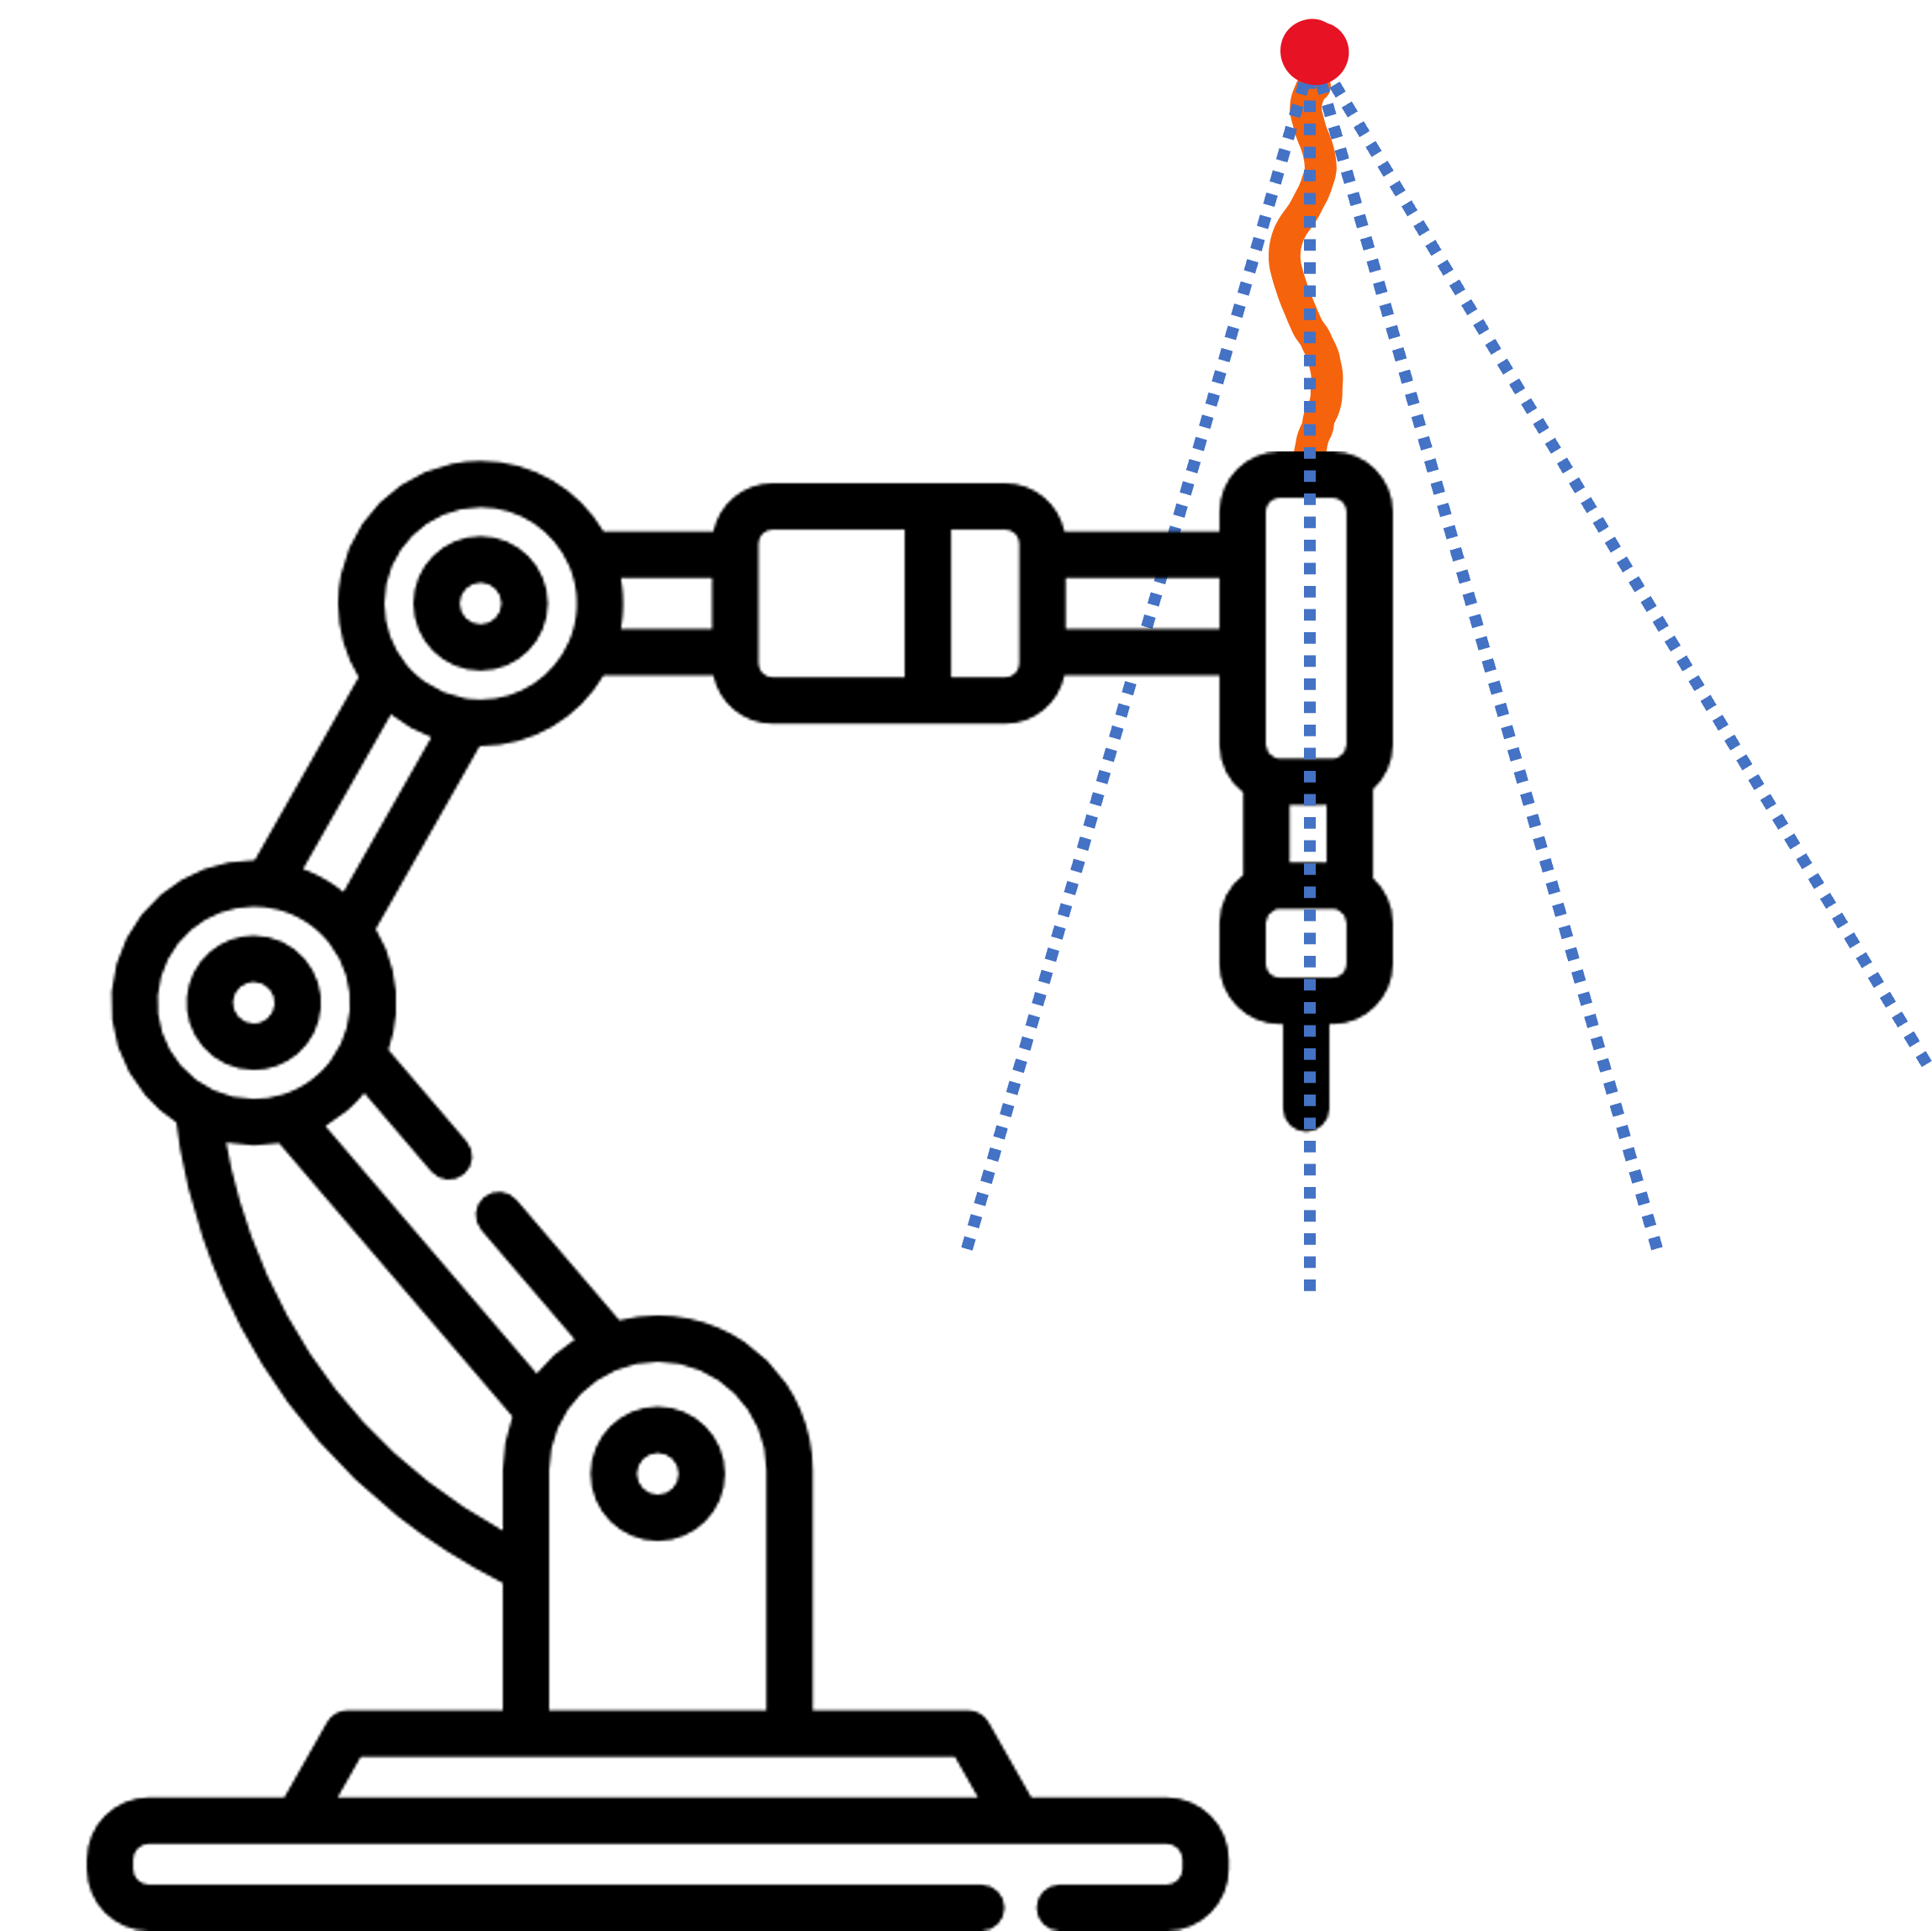
\includegraphics[width=.35\textwidth]{figures/angle.png}}}%
	\caption{Two examples for optimal alignments along a vector in 2D}%
	\label{OOPti}%
\end{figure}



To minimize the deviation from the optimal vector or vanishing point, the redundant \acrshort{DoF}s can be utilized. One approach is to analyze the deviation and track it over time, creating a time-series. Each element in this time-series can be squared or cubed, depending on the weight assigned to small and constant deviations versus large but short offsets. The time-series is then summed up to form a scalar value, which can be used to calculate the local score through the variation method. Table \ref{deviation} illustrates an example of how the scalar value is calculated. It is evident that when cubing the time series, more importance is placed on the larger deviations rather than small deviations.


\begin{table}[H]
	\centering
	\begin{tabular}{||l|c|c|c|c|c|c|c|c|l||}
		\hline
		Time-step:  & 1 & 2& 3& 4& 5& 6& 7& 8&  \\
		\hline
		Deviation:  & 1° & 2°& 2°& 2°& 3°& 10°& 0°& 2°&  \\
		\hline
		\hline
		Squared:  & 1 & 4& 4& 4& 9& 100& 0& 4& Sum: 126  \\
		Cubed:  & 1 & 8& 8& 8& 27& 1000& 0& 8& Sum: 1060  \\
		\hline
		\hline
		
	\end{tabular}
	
	\caption{From time-series of the deviation vector to scalar value}
	\label{deviation}
\end{table}

 

\subsection{Singularities}

In Chapter \ref{Singularity avoidance}, the concept of singularities in robotic systems is discussed. Singularities occur when the robot's joints align in a way that limits its motion by reducing one or more \acrshort{DoF}. To avoid singularities, it is important to optimize the boundary conditions in the redundant \acrshort{DoF}. The singularity analysis, as described in Table \ref{procesparameters}, can be represented either as a scalar value or as a time series that classifies each position based on its proximity to a singularity.

The scalar value can represent the overall smallest eigenvalue of every Jacobi matrix. For this, every pose needs to be analyzed. After calculating the Jacobi matrix, all eigenvalues encountered are examined, and only the smallest one is recorded and used to calculate the local score. This approach allows for an analysis of the overall toolpath rather than specific poses.

Alternatively, a time-series can be used where the determinant, not the eigenvalues, is recorded and stored. By analyzing this time series, it becomes possible to directly associate the robot's movements with its proximity to a singularity. This enables a more precise understanding of where the robot's motions are close to a singularity, allowing for subsequent optimizations. To transform the time series into a scalar value, the same threshold method described in Chapter \ref{VAJJ} can be applied.
  
  

\subsection{Torch Orientation in WAAM}
The torch orientation variable in \acrshort{WAAM}, similar to the cable routing orientation variable, analyzes the angle at which the welding torch is positioned during the process. This variable is specific to \acrshort{WAAM} and ensures that the torch is at the optimal angle for welding. Achieving material deposition in the direction of gravity is crucial for obtaining the best results. The orientation of the \acrshort{TCP}, which represents the welding torch tip, can be determined either through the forward kinematics approach or by extracting it directly from the G-code.

In both the forward kinematics approach and the G-code, the rotation is described as the rotation  around the A-, B-, and C-axes. However, the necessary information for torch orientation is simply the angle between the tilted Z-axis of the tool and the vector of gravity. To obtain this information, a dot product is performed between the rotation matrix and the Z-axis of the base coordinate system. This yields a vector corresponding to the tilted Z-axis of the tool. The enclosed angle can then be calculated using the scalar product. This step assumes that the defined bast coordinate system is oriented in a way that aligns the Z-axis parallel to the gravity vector. Figure \ref{tilt} gives a visual example in 2D on how the Z-axis of the tool is deviating from the vector of gravity.

\begin{figure}[H]
	\centerline{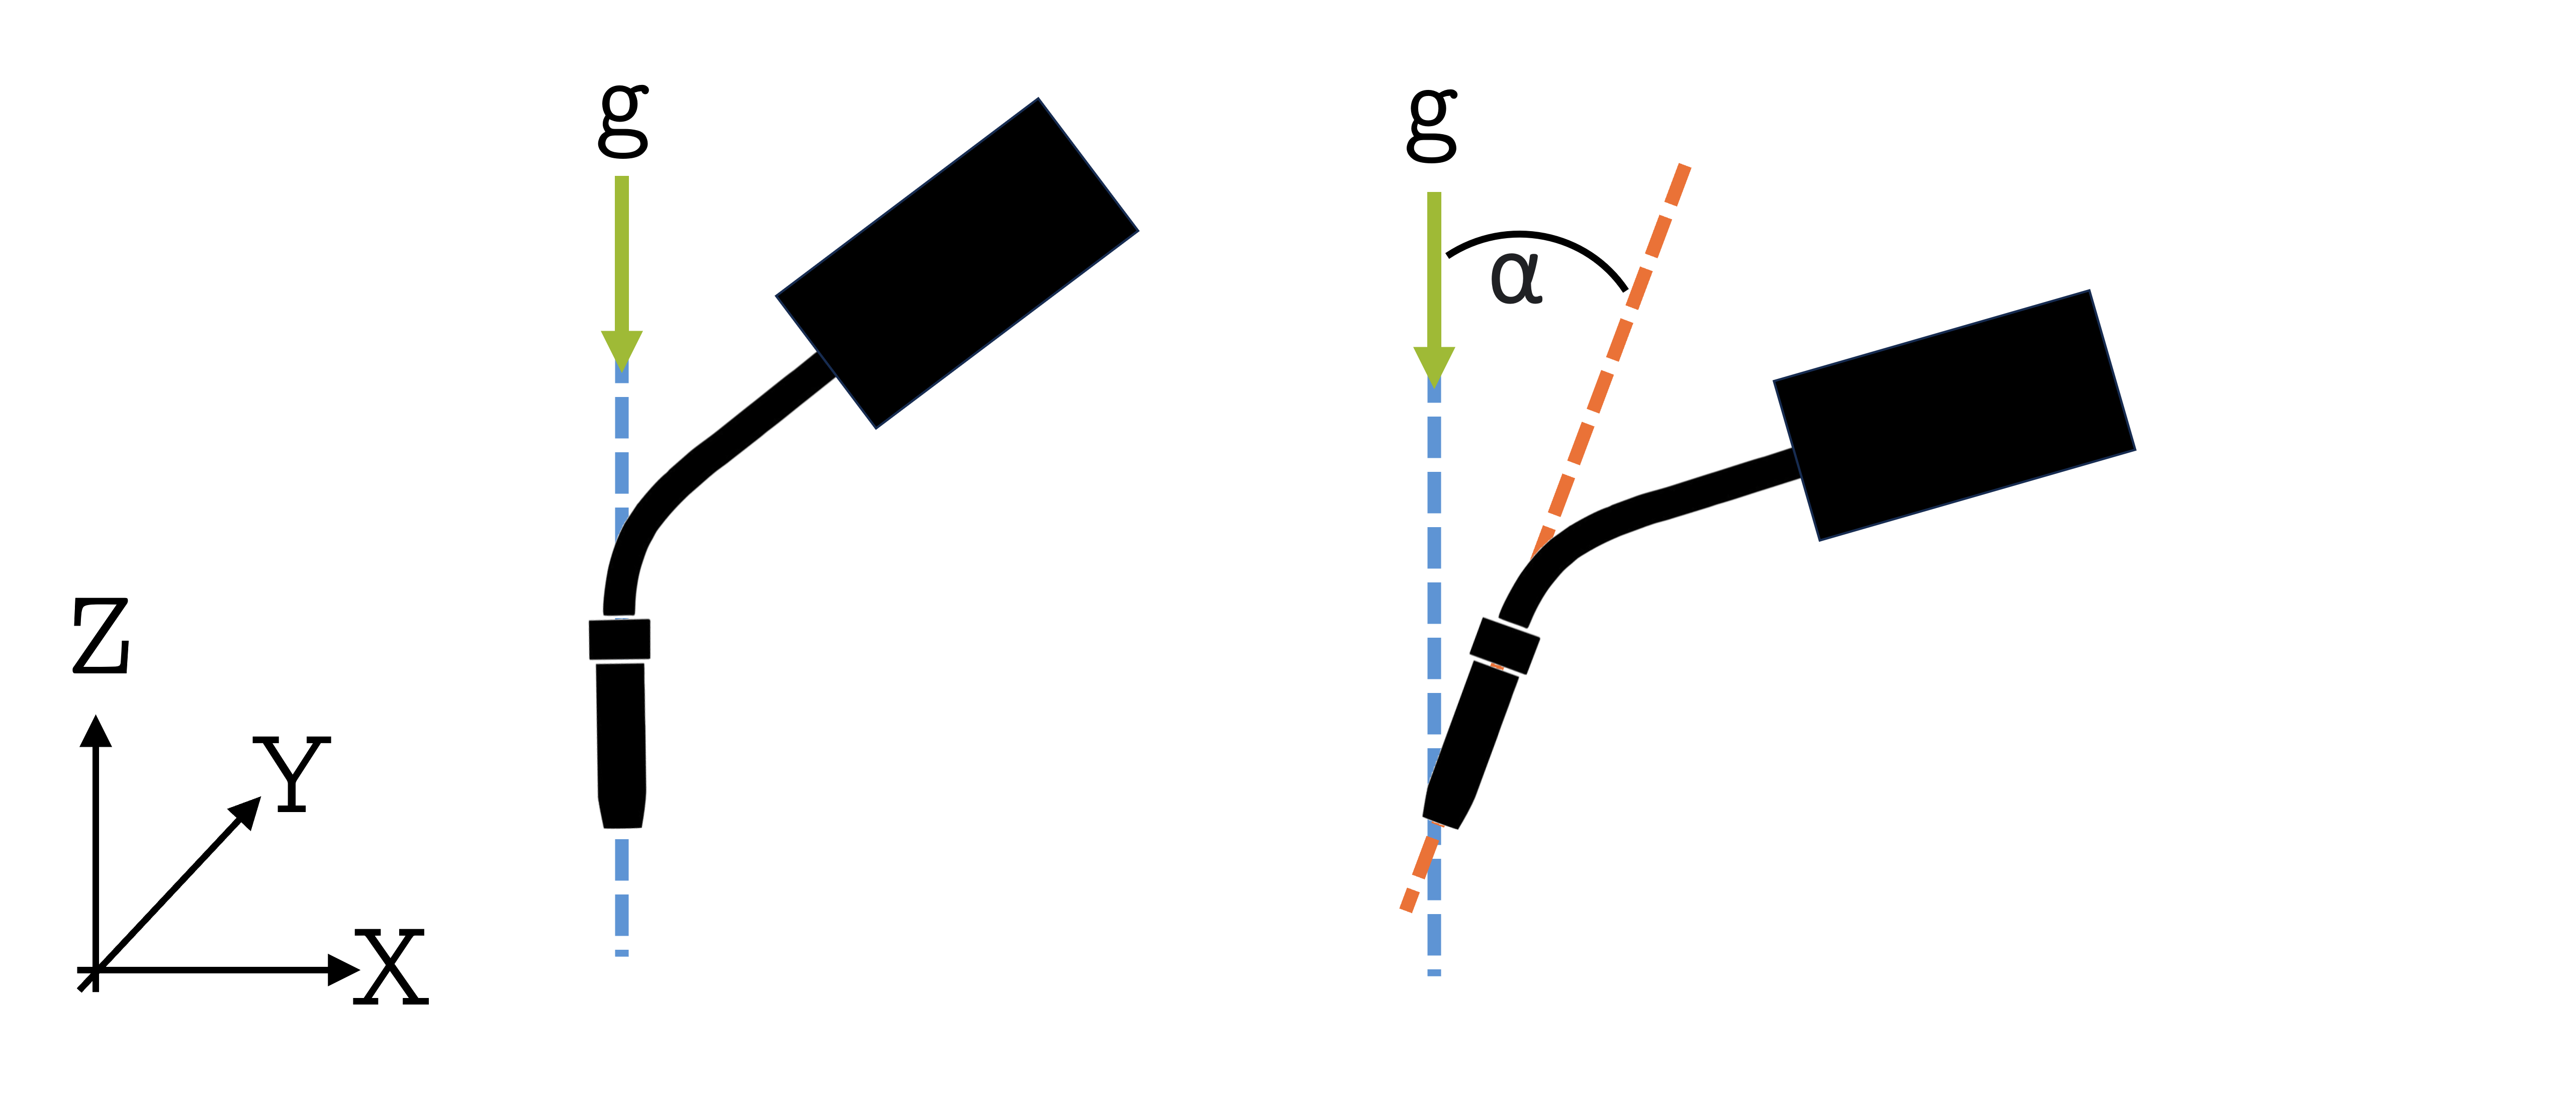
\includegraphics[width=.45\textwidth]{figures/ttilt.png}}
	\caption{Example of optimal and non-optimal tilt in the welding torch}
	\label{tilt}
\end{figure}

To quantify the torch orientation variable, it is recorded in a time-series format. To obtain a scalar value for this process variable, all the values can be squared, cubed, or subjected to other mathematical operations, and then summed up. This process is similar to the one described in Chapter \ref{RO} for the cable routing orientation variable.


\newpage
\section{Summary for Boundary Condition Evaluation}
Figure \ref{allflow} gives a summary and visual representation, in form of a flowchart, on how a toolpath with defined boundary conditions is evaluated by calculating the individual local scores for the process variables that can be influenced by the redundant \acrshort{DoF}s.

\begin{figure}[H]
	\centerline{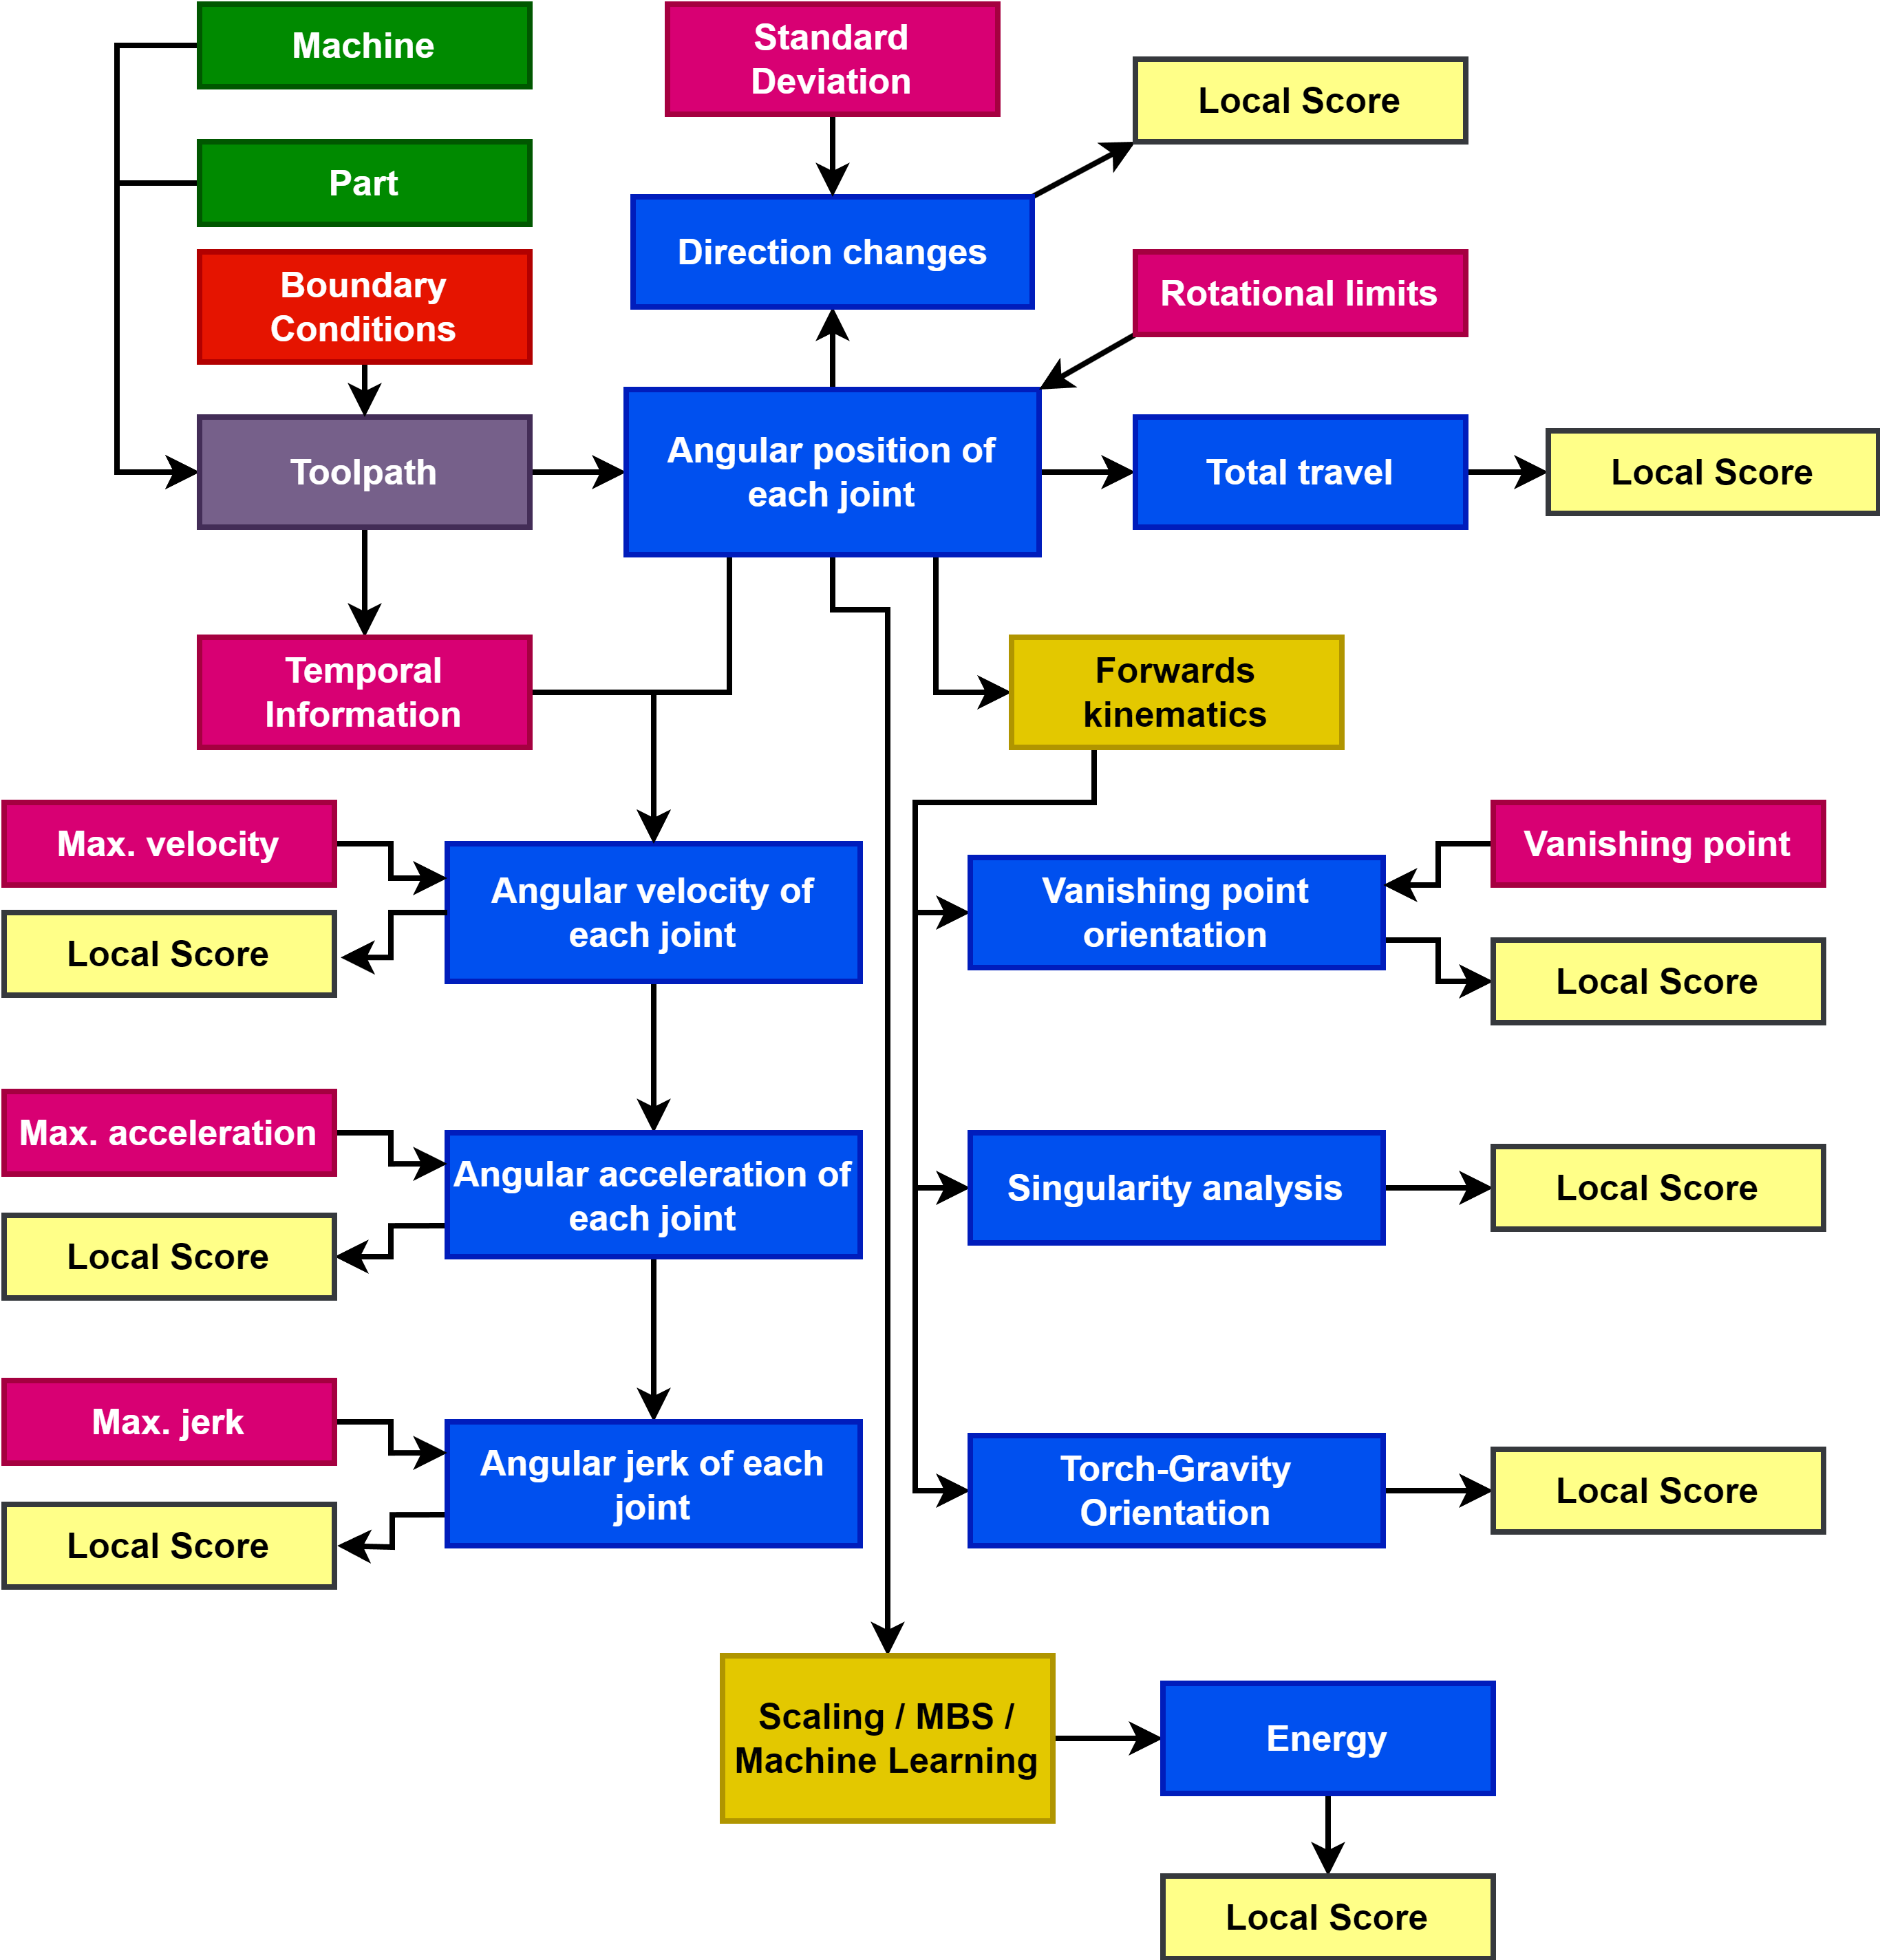
\includegraphics[width=1\textwidth]{figures/flowchart.png}}
	\caption{Evaluation of a toolpath}
	\label{allflow}
\end{figure}

\newpage
It is important to note that for a local score calculation the user defined importance values need to be multiplied with the local rating that results form the numerical values of the process variables. The local scores are then summed up to create the global score.

Figure \ref{grob} illustrates how a boundary condition for a toolpath can be evaluated. In this case, the toolpath is defined using only 5 \acrshort{DoF}s, including X-, Y- and Z-coordinates as wll as the rotation around the X- and Y-Axis. However, the rotation C around the Z-Axis, which is the axis of symmetry for the tool, is not defined and must be specified manually. Once this boundary condition is established, the joint positions are analyzed and individual variables, such as direction changes, can be extracted. In this example, the objective is to assess the optimality of a rotation angle of zero degrees of the C-axis. To calculate a local score, additional variations of the rotation around the C-Axis are analyzed. With the help of user-defined weights, the local ratings are weighted and summed up to form the global score for the boundary condition (see Chapter \ref{weights}).\newline


\begin{figure}[H]
	\centerline{\includegraphics[width=0.95\textwidth]{figures/grob.png}}
	\caption{Process of evaluating a defined boundary condition}
	\label{grob}
\end{figure}


\newpage
\section{General Methodology for Process Optimization}
So far only the analysis of a toolpath with set boundary conditions is discussed. In the following sections, two methods for optimizing boundary conditions towards a specific goal is presented. The main difference between these two methods lies in the different incorporation of a \acrshort{CAM} software.

It is important to note that optimizing certain process variables may have a direct negative impact on others. For example, optimizing the tools orientation towards a specific vanishing point can significantly increase the total number of direction changes in the joints. Therefore, the user must be aware of these cross-influences and adjust the weights accordingly.

\subsection{Optimization Without CAM Software in the Loop}\label{noCAMchap}

Figure \ref{noCAM} illustrates the process of optimizing the redundant \acrshort{DoF}s based on a predefined goal determined by weighing the process variables. In this method, the part and the manufacturing machine are fixed components that are loaded into the \acrshort{CAM} software. Before generating a toolpath, the redundant \acrshort{DoF}s must be set manually. These constraints can be set based on prior experience, as long as they do not lead to any "No-Go" exceptions caused by collisions or exceeding the joint limits.

When the toolpath is generated, it is defined in all available \acrshort{DoF}s of the manufacturing machine. This information is now in form of a G-code. To evaluate the set boundary conditions, the information from the G-code is extracted and the redundant \acrshort{DoF}s are varied, resulting in multiple toolpaths with multiple boundary conditions. In some cases, this variation simply involves varying the rotation around the Z-Axis, while keeping all the X-, Y- and Z-coordinates defined in the G-code, unchanged. In other cases, the redundant \acrshort{DoF}s involve the rotation and tilt of a rotary-tilt table. In such situations, every single coordinate in the G-code needs to be rotated around the tilting-axes of the rotary-tilt table. After obtaining the multiple toolpaths, each one is subjected to an inverse kinematics algorithm. This algorithm utilizes the machine's parameters, for example, arm length and joint sequence, to calculate the joint positions to reach every point in the different G-Codes. From these values, the score of the originally set boundary condition can be determined. By utilizing a external inverse kinematics approach, the \acrshort{CAM} software is not part of the optimization loop. This approach give  the user to work with any \acrshort{CAM} software.  

Following the score calculation, an optimization algorithm (see Chapter \ref{OA}) is employed to generate a new boundary condition for the redundant \acrshort{DoF}s. This cycle of optimization continues either for a predetermined number of iterations or a specified duration. Alternatively, a desired minimal score can be defined as the target, that the toolpath needs to achieve. Once the most optimal or close-to-optimal boundary condition is found, it is used as input for the \acrshort{CAM} software to validate that no collisions or other exceptions are triggered. After this validation process, the G-code can be utilized in production.

\begin{figure}[H]
	\centerline{\includegraphics[width=1\textwidth]{figures/noCAM.png}}
	\caption{Schematic process of optimization without CAM software in the loop}
	\label{noCAM}
\end{figure}

In this method, the optimization of boundary conditions occurs externally to the \acrshort{CAM} software. The \acrshort{CAM} software is solely utilized for generating the initial toolpath and validating the most optimal boundary condition that is returned by the optimization algorithm. The inverse kinematics process is performed outside of the \acrshort{CAM} software and can be implemented in various programming languages such as Python or C++. The same is applicable to the optimization algorithm.

The advantage of this approach is that the external algorithms are independent and can be easily exchanged or modified. It does not necessitate in-depth knowledge or access to the source code of the \acrshort{CAM} software. Therefore, any \acrshort{CAM} software can be utilized with this approach, providing flexibility and compatibility.    

However, it is important to note that one drawback of this approach is that the complete closure of the loop can only be achieved if the most optimal boundary condition can be automatically fed back to the \acrshort{CAM} software for the final validation. If there is no application programming interface (\acrshort{API}) available or accessible for the \acrshort{CAM} software, this step may need to be performed manually. This manual intervention can introduce additional time and effort into the optimization process.

Depending on the chosen optimization algorithm, it may be necessary to calculate multiple scores for multiple boundary conditions before generating a new suggestion. In this scenario, the variations in the redundant \acrshort{DoF}s can be utilized to calculate multiple scores relative to each other. These scores can then be used as input for the optimization algorithm, allowing for a more comprehensive evaluation and selection of the most optimal boundary condition. By considering multiple scores, the algorithm can effectively explore different possibilities and make informed suggestions for improving the boundary conditions.

Another drawback of this approach, is that for the variation of the redundant \acrshort{DoF}s the G-Code file is utilized. for that a dedicated software-program is necessary that can read the G-Code and adapt the individual coordinates accordingly. Another level of complexity can occur, if the G-Code is utilizing non-standard or user-defined commands. Many edge cases need to be considered before such a program is deemed save for production.       

Figure \ref{variation} illustrates the process of varying a simple toolpath. In this specific example, the toolpath is defined in six \acrshort{DoF}s, with the redundant \acrshort{DoF} being the rotation around the Z-axis. Initially, the toolpath is set at its original configuration with C = 0.0. To explore different possibilities, three variations of the toolpath are created by incrementing the rotation by 5 degrees for each variation. These variations allow for an examination of the impact of different orientations on the overall process. By systematically adjusting the rotation, the algorithm can evaluate the performance of each variation and suggest even better values.


\begin{figure}[H]
	\centerline{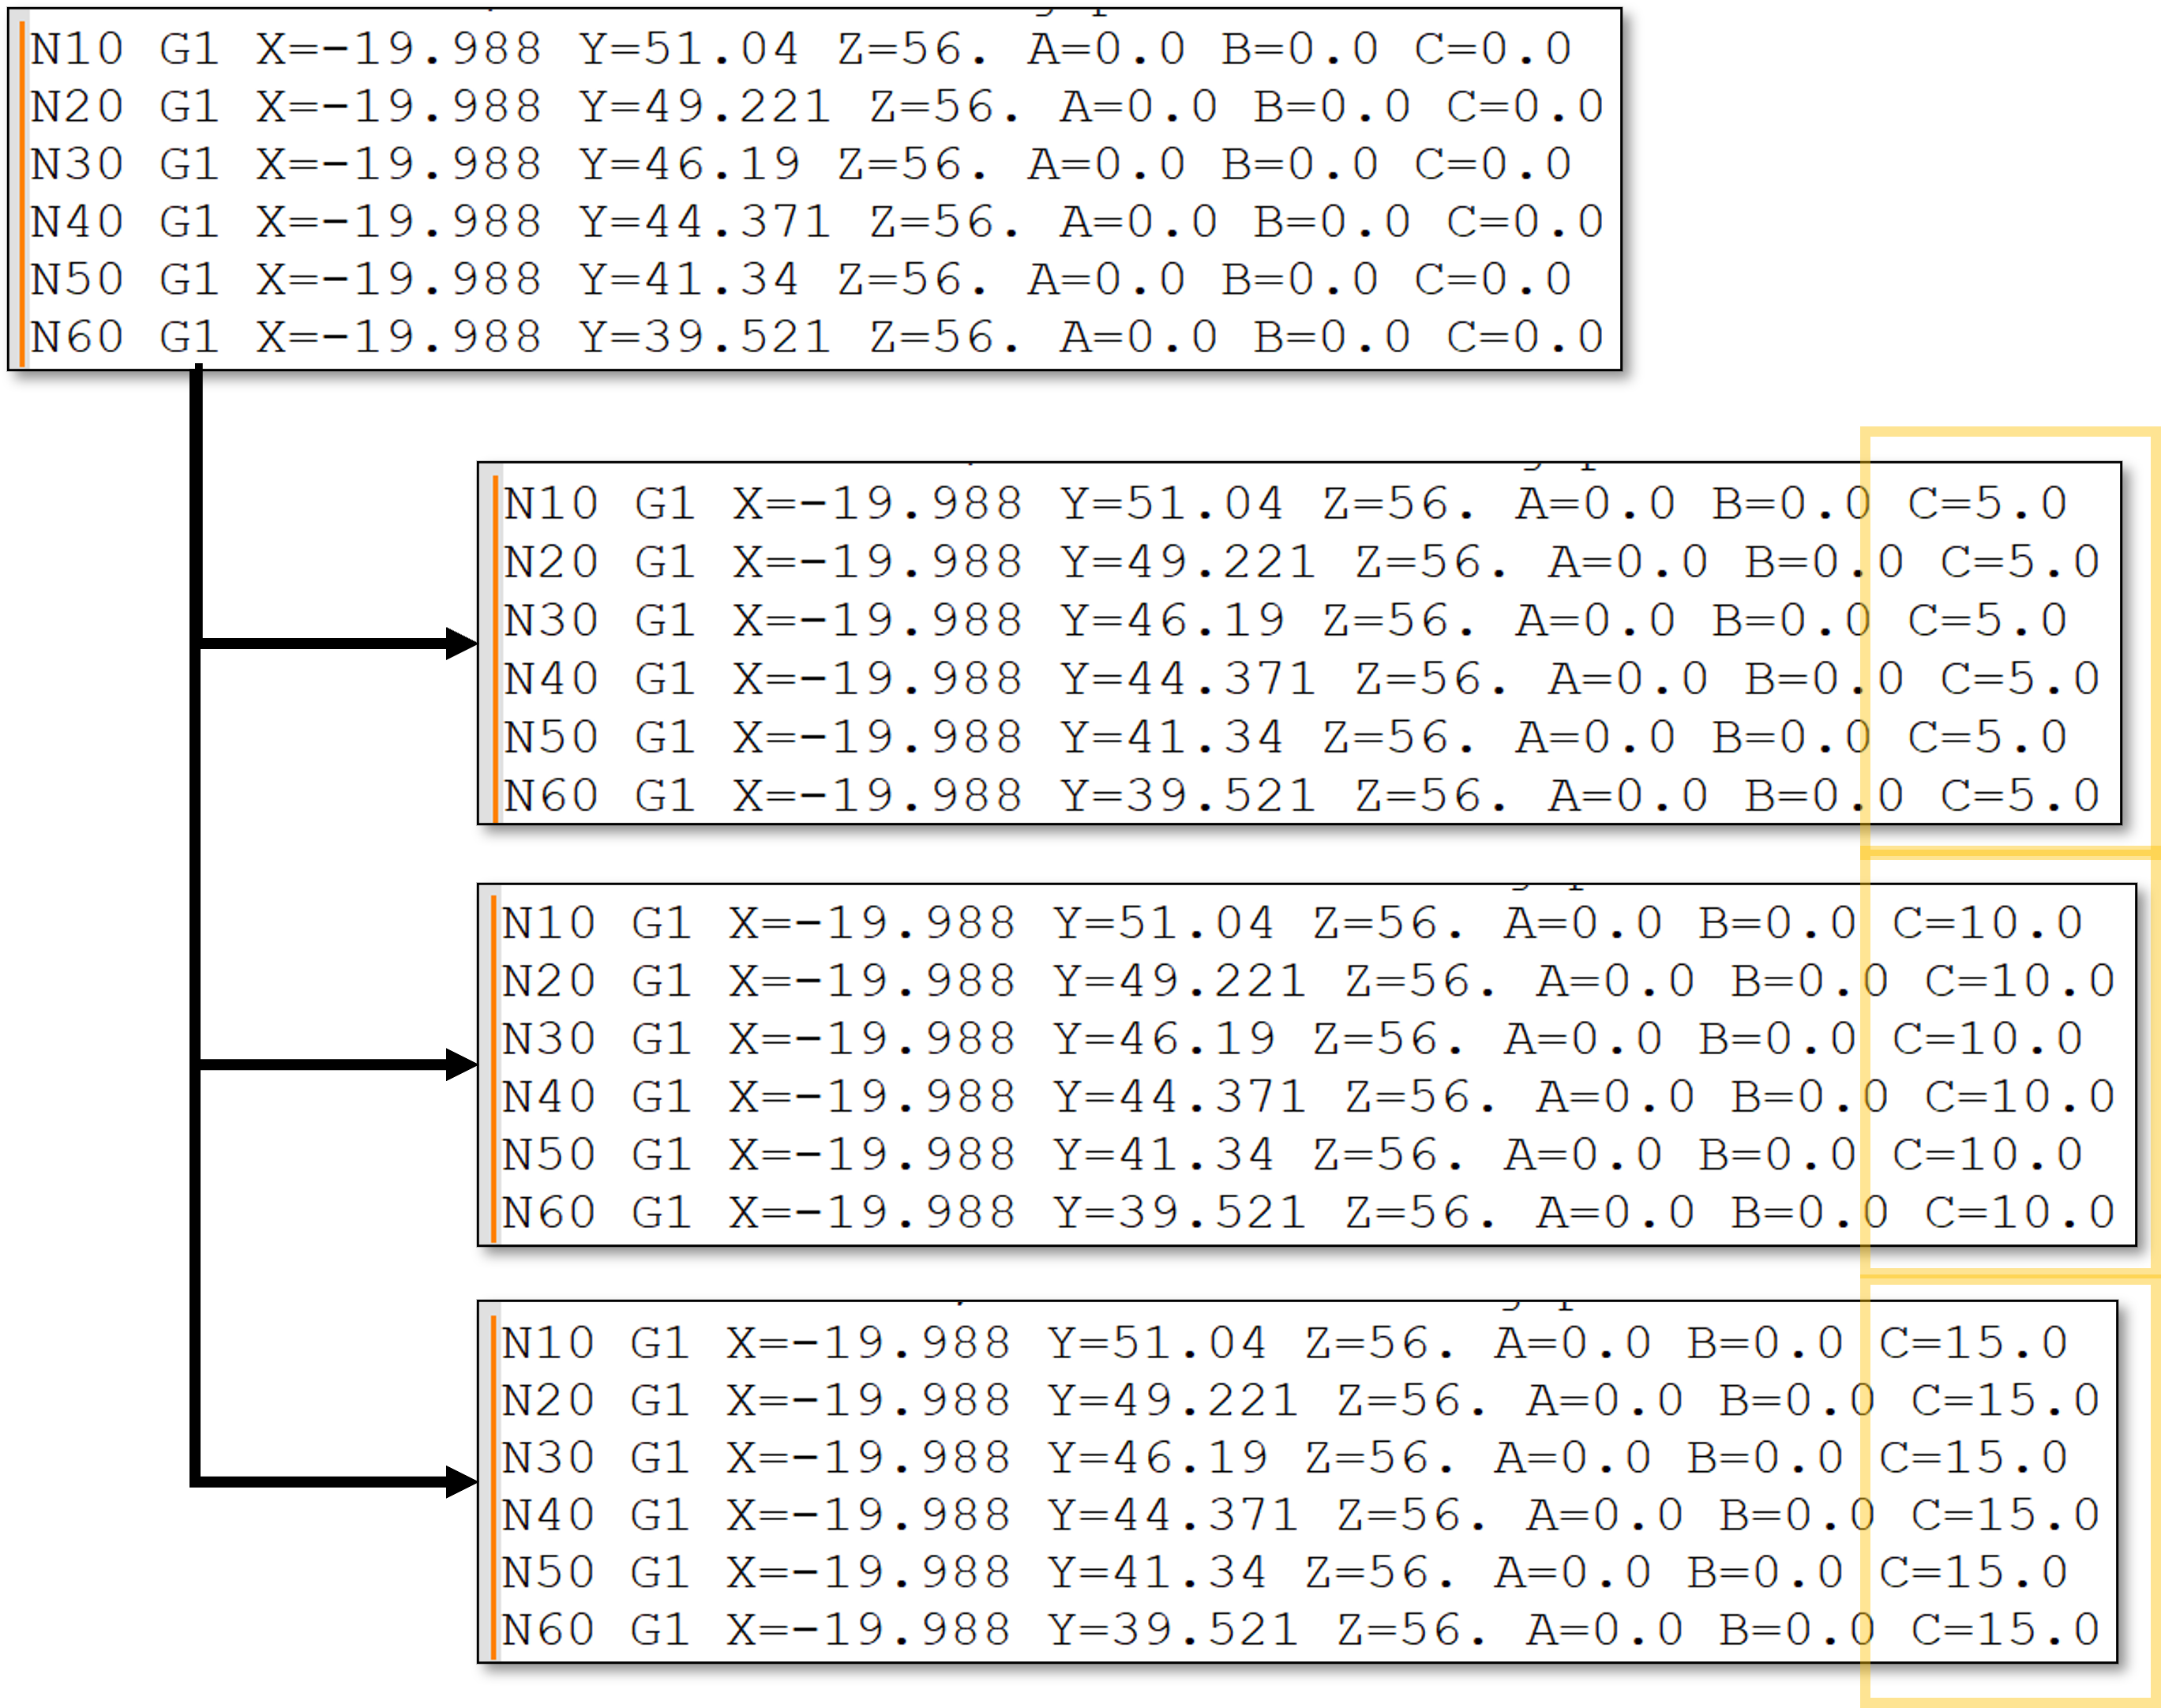
\includegraphics[width=0.9\textwidth]{figures/gcodevariation.png}}
	\caption{Variation of the redundant DoF in the G-code}
	\label{variation}
\end{figure}

\newpage
\subsection{Optimization Loop With CAM Software in the Loop}\label{CAMinloop}

The previously mentioned optimization approach in Chapter \ref{noCAMchap} describes a process that does not involve a \acrshort{CAM} software within the optimization loop. However, another method can be employed that directly incorporates a \acrshort{CAM} software into the optimization process and thus allows for seamless integration. By directly including the \acrshort{CAM} software, the optimization loop becomes more tightly knit, enabling seamless feedback and iteration between the toolpath generation and the optimization of constrains for the redundant \acrshort{DoF}s. This approach can significantly enhance the overall optimization process and significantly improves the quality and efficiency of the final toolpath.


In this method, the \acrshort{CAM} software plays a crucial role in the optimization process. It first generates the initial toolpath by automatically setting the redundant \acrshort{DoF} based on the given part geometry and machine configuration. Unlike traditional approaches, the \acrshort{CAM} software does not export G-code but utilizes its internal resources and algorithms to calculate the joint positions via a internal inverse kinematics algorithm. The optimization process is performed iteratively, involving multiple variations in the redundant \acrshort{DoF}s. Each variation generates a different toolpath, which in turn results in different joint positions of the manufacturing machine. The process variables are then analyzed to calculate a score that represents the quality of the toolpath. Figure \ref{CAMloop} shows the schematic representation of the optimization loop.\newline

 \begin{figure}[H]
 	\centerline{\includegraphics[width=1\textwidth]{figures/CAMloop.png}}
 	\caption{Schematic process of optimization with CAM software in the loop}
 	\label{CAMloop}
 \end{figure}



The optimization algorithm, seamlessly integrated within the \acrshort{CAM} software, utilizes the obtained scores to propose a new setting for the redundant \acrshort{DoF}s. This new setting aims to improve the toolpath and optimize the process variables further. The iteration continues until a defined score or a predetermined number of iterations is reached, indicating that the optimization loop has converged.
Once the optimization loop is terminated, the \acrshort{CAM} software exports the G-code with the best-found boundary conditions, representing the optimized toolpath.

The advantage of this approach lies in leveraging the \acrshort{CAM} software's specialized capabilities and features for toolpath generation and optimization. By directly integrating with the software, the optimization process becomes more efficient and streamlined, eliminating the need for external scripts or algorithms.

However, a significant disadvantage of this method is the requirement for access to the source code of the \acrshort{CAM} software to add the optimization algorithm and the specific post-processor that calculates the joint positions. Adding the necessary features and functionalities necessitates modifying the software, which may not be feasible or practical in all situations. For that reason, this approach has to be implemented by the provider of the \acrshort{CAM} software. 